
%%%%%%%%%%%%%%%%%%%%%%%%%%%%%%%%%%%%%%%%%%%%%%%%%%%%%%%%%%%%%%%%%%%%%%%%%%%%%%%
%                                                                              %
%                                 Bachelorarbeit                               %
%                        Universit�t der Bundeswehr M�nchen                    %
%                                                                              %
%%%%%%%%%%%%%%%%%%%%%%%%%%%%%%%%%%%%%%%%%%%%%%%%%%%%%%%%%%%%%%%%%%%%%%%%%%%%%%%%

\documentclass[a4paper							% Papierformat: A4
							 ,titlepage						% Titelseite						 
							 ,ngerman							% Neue Rechtschreibung verwenden
%							 ,draft								% auskommentieren, um zu lange/kurze Zeilen zu finden
							 ,bibliography=totoc 	% Literaturverzeichnis ins Inhaltsverzeichnis aufnehmen
							 ]
%							 {scrartcl} 					% erlaubt "section", "subsection", ...
							 {scrreprt} 					% statt scrartcl, zus�tzliche Gliederungsebene "chapter"
							 
\usepackage[ngerman]{babel}		% Neue Rechtschreibung verwenden 
\usepackage[latin1]{inputenc}
\usepackage[T1]{fontenc}
\usepackage{lmodern}					% H�bschere Schriftart als Standard
\usepackage{microtype}				% Verbesserter Textsatz

\usepackage{graphicx} 				% Bilder einbinden
\usepackage{tabularx} 				% Tabellen mit definierbarer Breite
\newcolumntype{C}[1]{>{\centering\arraybackslash}p{#1}} % zentriert mit Breitenangabe
\usepackage{booktabs}					% h�bschere Tabellen
\usepackage{xcolor}
\usepackage{multirow}
\usepackage{caption}
\usepackage{longtable}
\usepackage{amssymb}
\usepackage{enumitem}
%\usepackage[hyphens,spaces,obeyspaces]{url}
\usepackage[titletoc,title]{appendix}	

% Seitenstil definieren
\usepackage{scrpage2}
\pagestyle{scrheadings}
\automark{section}						% Kolumnentitel automatisch aus den "Sections" bestimmen

\usepackage[hyphens]{url}
\renewcommand{\UrlBreaks}{\do\a\do\b\do\c\do\d\do\e\do\f\do\g\do\h\do\i\do\j\do\k\do\l\do\m\do\n\do\o\do\p\do\q\do\r\do\s\do\t\do\u\do\v\do\w\do\x\do\y\do\z\do\A\do\B\do\C\do\D\do\E\do\F\do\G\do\H\do\I\do\J\do\K\do\L\do\M\do\N\do\O\do\P\do\Q\do\R\do\S\do\T\do\U\do\V\do\W\do\X\do\Y\do\Z\do\-}

\usepackage{natbib}
\setlength{\bibsep}{7.0pt}
%\usepackage[hyphenbreaks]{breakurl}

%%%%%%%%%%%%%%%%%%%%%%%%%%%%%%%%%%%%%%%%%%%%%%%%%%%%%%%%%%
% QUELLCODE-STUFF
%%%%%%%%%%%%%%%%%%%%%%%%%%%%%%%%%%%%%%%%%%%%%%%%%%%%%%%%%%


\usepackage{listings}

\lstset{language=XML,
	breaklines=true,
	frame=lrb,
	keywordstyle=\color{blue},
	commentstyle=\color{gray},
	identifierstyle=\color{black},
	stringstyle=\color{red},
	numbers=left,
	numbersep=-10pt,               
	numberstyle=\tiny\color{black},
	xleftmargin=0.31em,
	xrightmargin=-0.235em,
	tabsize=4,
	emph={VMware,Virtual,Platform,Inc,computer-vm,Icon,name,Virtualization,Chassis,vmware,computer,vm},
	emphstyle={\color{red}},
	%otherkeywords={'0', '1'}
	morekeywords={VMware}
}

\DeclareCaptionFont{white}{\color{white}}
\DeclareCaptionFormat{listing}{\parbox{\textwidth}{\colorbox{gray}{\parbox{\textwidth}{#1#2#3}}\vskip-4pt}}
\captionsetup[lstlisting]{format=listing,labelfont=white,textfont=white}




%%%%%%%%%%%%%%%%%%%%%%%%%%%%%%%%%%%%%%%%%%%%%%%%%%%%%%%%%%
% ENDE QUELLCODE-STUFF
%%%%%%%%%%%%%%%%%%%%%%%%%%%%%%%%%%%%%%%%%%%%%%%%%%%%%%%%%%


\PassOptionsToPackage{hyphens}{url}

% Links im fertigen PDF erstellen
\usepackage[% hyperref immer als letztes (!) Paket einbinden!						
						pdfauthor={Marcel Antzek}
						,pdfsubject={Bachelorarbeit}
						,pdftitle={Evaluation und Implementierung versteckter Kan�le in IP-basierten Protokollen im Kontext von Malware C\&C-Verkehr}
						,plainpages = false		% notwendig wg. r�mischer und arabischer Seitenzahlen
						,pdfpagelabels = false %	auch im AR zwischen ii und 2 unterscheiden!?
					%	,implicit = false
						,breaklinks = true		% Links umbrechen
						,colorlinks = true		% Links f�rben, statt umranden
						,linkcolor  = black		% interne Links
						,citecolor  = black		% Zitate
						,menucolor  = black		% Links im Inhaltsverzeichnis
						,urlcolor   = black		% URLs blau f�rben (blue)
					]{hyperref}



%%%%%%%%%%%%%%%%%%%%%%%%%%%%%%%%%%%%%%%%%%%%%%%%%%%%%%%%%%%%%%%%%%



\begin{document}
	
	\pagenumbering{Roman}
	% Deckblatt
	%%%%%%%%%%%%%%%%%%%%%%%%%%%%%%%%%%%%%%%%%%%%%%%%%%%%%%%%%%%%%%%%%%%%%%%%%%%%%%%%
%                                                                              %
%                                 Bachelorarbeit                               %
%                        Universit�t der Bundeswehr M�nchen                    %
%                                                                              %
%%%%%%%%%%%%%%%%%%%%%%%%%%%%%%%%%%%%%%%%%%%%%%%%%%%%%%%%%%%%%%%%%%%%%%%%%%%%%%%%

\begin{titlepage}
	\centering
	
	
\includegraphics[width=0.5\textwidth]{unibwm_signet}
	\\
	\vspace{2cm}
  \LARGE{\textsf{Projektarbeit}}
  \\
  \vspace{2cm}
  \LARGE{\textsf{\textbf{Entwurf, Implementierung und Evaluation einer prototypischen L�sung f�r Bestell- und Bezahlprozesse auf Blockchain-Basis in mittelst�ndischen Unternehmen}}}
  \\
  \vfill
  \textsf{
    \begin{normalsize}
    \begin{tabular}{ll}
      Eingereicht von: 	& Marcel Antzek, Bastian K�hnel,\\
                       	& Felix Leber, Christopher Lemm,\\
                      	& S�nke R�ckwardt, Daniel Schick\\
                      	\\
      Betreuung: 	& M.Sc. Tim Reimers\\\\ 	
      Modul: 	& IT-Management\\ 
       			& Modulnummer 1047\\ 			                     
												\\	        
												\\		 
	  Abgabedatum: 			& \textcolor{black}{23. M�rz 2018}\\
    \end{tabular}        
    \end{normalsize}    
  }
  \\
  \vfill
  \normalsize{\textsf{Universit�t der Bundeswehr M�nchen\\Fakult�t f�r Informatik\\Institut f�r Technische Informatik}}
  
\end{titlepage}


	
\thispagestyle{empty}
\clearpage
\hbox{}\newpage
	
	% Abstract
	
\subsubsection{\label{chap0:abstract}Abstract}

Im Verlauf dieser Arbeit wird die Blockchain-Technologie beschrieben. Ziel ist es durch diese Technologie Chancen und Risiken f�r die IT erfassen und bewerten zu k�nnen. Hierzu wird zun�chst eine Machbarkeitsstudie und eine Risikoanalyse f�r ein entsprechendes Tool angefertigt. Anschlie�end wird die Blockchain-Technologie f�r einen spezifischen Anwendungskontext in einem Demonstrator (WebApp) umgesetzt. Au�erdem werden Interviews mit kleinen Unternehmen des Gastronomiesektors durchgef�hrt, um festzustellen, wie diese die M�glichkeiten der Technologie wahrnehmen und den Demonstrator bewerten. Diese Ergebnisse werden zusammengefasst und ausgewertet.
	
\thispagestyle{empty}
\clearpage
\hbox{}\newpage

	% Inhaltsverzeichnis
	\tableofcontents
	\newpage
	

	% Abbildungsverzeichnis
	\listoffigures
	

	% Tabellenverzeichnis
	
\thispagestyle{empty}
\clearpage
\hbox{}\newpage
	\listoftables
	\addcontentsline{toc}{section}{Tabellenverzeichnis}

	%Listings-�bersicht
	
\thispagestyle{empty}
\clearpage
\hbox{}\newpage
	\lstlistoflistings
	\addcontentsline{toc}{section}{Listings}

	% Abk�rzungen
	
\thispagestyle{empty}
\clearpage
\hbox{}\newpage
	%%%%%%%%%%%%%%%%%%%%%%%%%%%%%%%%%%%%%%%%%%%%%%%%%%%%%%%%%%%%%%%%%%%%%%%%%%%%%%%%
%                                                                              %
%                                 Bachelorarbeit                               %
%                        Universit�t der Bundeswehr M�nchen                    %
%                                                                              %
%%%%%%%%%%%%%%%%%%%%%%%%%%%%%%%%%%%%%%%%%%%%%%%%%%%%%%%%%%%%%%%%%%%%%%%%%%%%%%%%

\section*{Abk�rzungsverzeichnis}

%\manualmark           % Kolumnentitel anpassen
\markright{Abk�rzungsverzeichnis}

\addcontentsline{toc}{section}{Abk�rzungsverzeichnis}


\vspace{\baselineskip}

\begin{tabularx}{\linewidth}{p{3cm}X}

ABI & Application Binary Interface\\
%Bitkom & Bundesverband Informationswirtschaft, Telekommunikation und neue Medien e.V.\\
BTC & Bitcoin\\
DApp & Decentralized Application\\
ETH & Ethereum\\
EVM & Ethereum Virtual Machine\\
ID & Identifikator\\
IT & Informations-Technologie\\
P2P & Peer-to-Peer \\
SWOT & Strengths, Weaknesses, Opportunities und Threats\\
UML & Unified Modeling Language\\



\end{tabularx}

	
	
\thispagestyle{empty}
\clearpage
\hbox{}\newpage
	\pagenumbering{arabic} 
	\renewcommand\thechapter{\arabic{chapter}} 
	\setcounter{chapter}{0} 

	% Einleitung
	\chapter{Einleitung}

	Diese Arbeit wird eine Abhandlung �ber die Blockchain beziehungsweise ihrer Anwendungsm�glichkeit in spezifischem Kontext sein. Genauer werden Einsatzgebiete beleuchtet und Chancen die sich f�r die IT und somit auch die Nutzer daraus ergeben. Es werden aber auch m�gliche Risiken aufgezeigt. 

	\section{Motivation}
	
		\label{chap:1einleitung}
		
		Wir leben im 21. Jahrhundert, indem die Bedeutung von Daten immer mehr zunimmt. Eine Vielzahl von Ger�ten verf�gt mittlerweile �ber einen Speicher irgend einer Form und auch besonders die Anzahl der Ger�te, welche vernetzt operieren nimmt drastisch zu. Der daraus resultierende Zuwachs des Wertes von Daten geht soweit, dass in einem Artikel "`der Zeit"' sogar soweit gegangen wird davon zu sprechen, dass Daten das Gold des 21. Jahrhunderts seien \cite{gd21jh}. H�ufig gibt es f�r solche Daten keinen zentralen IT-Dienst, weshalb diese dezentral beispielsweise mittels P2P-Netzen umgesetzt werden. Was das genau bedeutet und wie so etwas funktioniert wird in Kapitel \ref{subsec:p2p} beschrieben. In vielen F�llen ist die Korrektheit dieser Daten von essenzieller Bedeutung f�r verschiedenste Parteien.  Betrachtet man das Beispiel, dass 2 Parteien ein Vertrag in .PDF-Form vorliegen haben. Sagt die eine Datei nun, dass beispielsweise eine 1000 Euro Zahlung f�llig wird und die andere sagt es w�rden 2000 Euro f�llig, birgt dies ein deutliches Konfliktpotential. Ohne eine �berpr�fungsm�glichkeit ist hier ein Streit vorprogrammiert und eine L�sung l�sst sich m�glicherweise nur schwer erzielen. Sind diese Daten nun aber mit einem Mechanismus versehen, der sie auf Echtheit und Richtigkeit pr�fen kann ist es m�glich potentielle Konflikteskalationen zu vermeiden. Die beiden Datens�tze k�nnten einem unabh�ngigen Gericht vorgelegt werden und anhand dieser Mechanismen k�nnte Recht gesprochen werden. Der Streit w�re gel�st.
		
		Ein solcher Mechanismus zum Nachweisen der Echtheit und Richtigkeit k�nnte beispielsweise eine Blockchain sein. Sehr grob beschrieben ist die Blockchain ein Mechanismus, der vergangene Informationen beziehungsweise Versionen in seiner sogenannten Headerinformation anzeigt beziehungsweise referenziert. Neue Informationen werden in sogenannten Bl�cken angef�gt, wodurch der tats�chliche Informationsgehalt der Blockchain stetig w�chst. Dieser Mechanismus wird in Abbildung \ref{BC} veranschaulicht, wobei "`ABC"' als Name der Version zu verstehen ist. Eine genauere und technischere Beschreibung wird ebenfalls in Kapitel \ref{chap:2grundlagen} folgen.
		\newpage
		
		\begin{figure}[htbp]
			\centering
			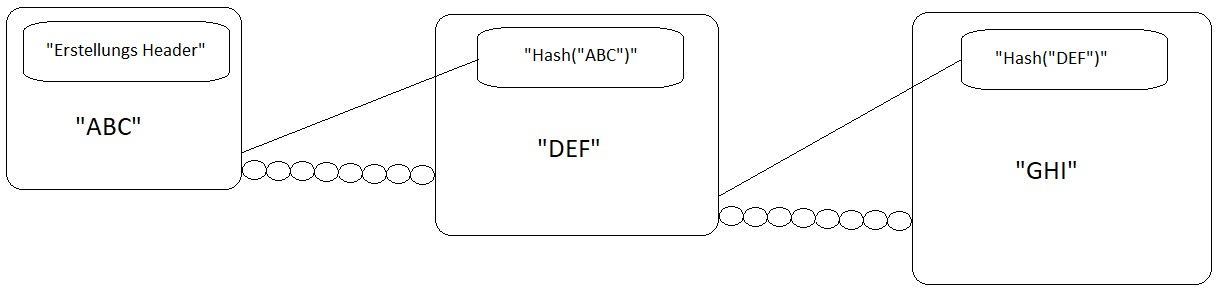
\includegraphics[keepaspectratio,width=\textwidth]{Bilder/blockchain.jpg}
			\caption{Beispieldarstellung Blockchain}
			\label{BC}
		\end{figure}
		
		Die im wohl bekanntesten Anwendungsf�lle der Blockchain-Technologie sind wohl die Kryptow�hrungen. Allen voran ist hier der sogenannten Bitcoin zu nennen. Bitcoin ist eine 2009 unter dem Pseudonym Satoshi Nakamoto, �ber dessen wahre Identit�t oder Identit�ten bis heute  nur spekuliert werden kann, ver�ffentlichte Kryptow�hrung. Bitcoin war laut Statista (Stand 2017) die mit deutlichem Abstand dominante Kryptow�hrung \cite{kwrank}. Als n�chstes zu nennen und Bitcoin auf Rang 2 der Krypow�hrungen folgend ist Ethereum, welches im Jahr 2013 von Vitalik Buterin vorgestellt wurde und im Jahr 2015 erschien. Ethereum selbst ist eigentlich nicht die Kryptow�hrung, sondern das System, welches mit der W�hrung ETH arbeitet. Der Unterschied zwischen Bitcoin und Ethereum ist, dass Ethereum zus�tzlich sogenannte "`Smart Contracts"' verarbeitet, welche so viel wie "`Intelligente Vertr�ge"' bedeuten. Die beiden bisher genannten Beispiele unterliegen im Vergleich zu "`echten"' W�hrungen keiner zentralen Verwaltung wie beispielsweise Banken, sondern ihr Wert bestimmt sich zu 100\% aus Angebot und Nachfrage. Weniger bekannt, aber nicht weniger relevant ist das Hyperledger Project. Hierbei handelt es sich nicht um eine Blockchain an sich, sondern eher um eine Ansammlung von Open Source Blockchain Tools. Diese Tools besch�ftigen sich damit Daten �berpr�fbar und sicher zu machen. Auch bietet Hyperledger einige Frameworks zum Entwickeln eigener Blockchain Tools an, um diese weiter zu verbreiten. Die einigen wohl schon bekannten Logos der drei Angesprochenen sind in Abbildung \ref{diedrei} zu sehen.
		
		\begin{figure}[htbp]
			\centering
			
\includegraphics[keepaspectratio,width=\textwidth]{Bilder/die3vorgestellten.jpg}
			\caption{Die drei angesprochenen Blockchain-Anwendungen}
			\label{diedrei}
		\end{figure} 
		
	\section{Aufbau des Dokumentes}
	
		In Kapitel \ref{chap:1einleitung} wurde eine Einf�hrung in das Thema Blockchain gegeben. In Kapitel \ref{chap:2grundlagen} wird auf die theoretischen Grundlagen eingegangen und jene erl�utert. Zun�chst wird dort auf Kryptohashes eingegangen. Anschlie�end wird allgemein P2P (Peer-to-Peer) erl�utert und darauf folgend dezentrale Netze erkl�rt. Danach wird Asymmetrische Kryptographie betrachtet und schlie�lich mit der genaueren Erl�uterung des Begriffs Kryptow�hrung abgeschlossen. In Kapitel \ref{chap:3methodik} wird ddas methodische Vorgehen in dieser Arbeit erl�utert. Dazu geh�ren unter anderem die Durchf�hrung von Interviews und einer Machbarkeitsstudie. In Kapitel \ref{chap:4szenario} wird zun�chst eine betriebswirtschaftliche Kontextualisierung durch gef�hrt. Anschlie�end wird ein Fallbeispiel geliefert und verschiedene Use-Cases aus dem Bereich der Gastronomie aufgezeigt. In Kapitel \ref{chap:5proto} wird ein entworfener Prototyp vorgestellt sowie f�r diesen ben�tigte  beziehungsweise durch ihn durchgef�hrte Smart Contracts erl�utert. Die Arbeit schlie�t mit dem Kapitel \ref{chap:6fazit} einem Fazit.	
	
	\section{Wissenschaftliche Forschungsfragen}\label{sec:fragen}
		
		Die Analyse des komplexen und umfangreichen Problemkontextes kann nur auf Basis einer grobgranularen Vordifferenzierung in st�rker fokussierte Teilaspekte realisiert werden. Zur Repr�sentation der initial identifizierten Problembereiche sollen im Verlauf des folgenden Abschnittes wissenschaftliche Forschungsfragen formuliert werden, aus deren Bearbeitung die Identifikation von Malware-Methoden zur Detektion virtualisierter Laufzeitumgebungen sowie die \mbox{Konzeption von korrespondierenden Verschleierungsma�nahmen resultiert.} \\
		
		\noindent\textbf{1. Welche Verfahren zur Analyse von Malware-Implementierungen existieren und welche Relevanz besitzen virtuelle Systeme in diesem Kontext?}\\
		
		\begin{addmargin}[1em]{0em}
			\noindent Das Verst�ndnis wesentlicher Parameter von Komposition und Funktionalit�t konkreter Malware-Derivate erfordert die extensive Analyse exemplarischer Implementierungen. Hierbei lassen sich divergente Analyseans�tze differenzieren, welche beispielsweise die dedizierte Quellcode-Analyse oder die dynamische Simulation des Malware-Verhaltens priorisieren. Um die potentiell unkontrollierbare Infektion von weiteren Elementen in produktiven Systemumgebungen zu vermeiden, werden dabei in der Regel virtuelle Systeme zur gefahrlosen Examination der Schadsoftware instrumentalisiert. Die kontinuierliche Weiterentwicklung im Kontext der Virtualisierung offeriert im Vergleich zur manuellen Analyse auf physischen Produktivsystemen weitere Vorteile, deren Beitrag zur \makebox[\linewidth][s]{Realisierung von Malware-Analysen in einem dedizierten Abschnitt diskutiert wird.}  \\
		\end{addmargin}	
		
		\noindent\textbf{2. Welche systemspezifischen Indizien werden von aktuellen Malware-\\\noindent Implementierungen zur Detektion virtueller Systemumgebungen eingesetzt?}\\
		
		\begin{addmargin}[1em]{0em}
			\noindent Auf Basis einer initialen Pr�sentation der von Virtualisierungs-Implementierungen induzierten System-Anomalien werden diese anhand der intern verwendeten Methodik einer grobgranularen Kategorisierung unterzogen. Prim�r wird hierbei zwischen hardwareorientierten Realisierungsans�tzen und softwarebasierten Konzepten differenziert, wobei final eine dedizierte Evaluation der identifizierten Detektionsans�tze hinsichtlich ihrer Realisierbarkeit in produktiven Systemkontexten durchgef�hrt wird. So sind insbesondere die im Rahmen verdeckter Initialkompromittierungen verwendeten Datens�tze quantitativ zu limitieren, um die kapazit�re Belastung der zu kompromittierenden Systeme und die hierdurch induzierten Anomalien zu minimieren. Auch dieser mitunter nicht unkritische Aspekt soll im Rahmen einer Kompromissfindung zwischen dem Leistungsumfang der Detektionsmethoden und ihrer Verdecktheit ber�cksichtigt werden. \\
		\end{addmargin}
		
		\noindent\textbf{3. Welche Methoden und Verfahren k�nnen zur Optimierung der in einem virtuellen System generierten Analyse-Resultate eingesetzt werden?}\\
		
		\begin{addmargin}[1em]{0em}
			Ein wesentliches Element zur Optimierung von Analyse-Resultaten im Kontext virtualisierter Systeme ist die Konfiguration des Systems zur m�glichst realit�tsnahen Emulation einer produktiven Umgebung. Auf diese Weise k�nnen die im Rahmen der vorhergehenden Analyse identifizierten Detektionsmechanismen von Malware-Implementierungen get�uscht werden, wodurch final die Analyse des vollst�ndigen Funktionalit�tsumfangs erm�glicht wird.
			Unter Ber�cksichtigung der Diversit�t moderner Malware-Realisierungen sind weiterhin Konzepte zu erarbeiten, welche eine m�glichst adaptive Anpassung der identifizierten Optimierungsmethoden an die ver- \makebox[\linewidth][s]{schiedenen Implementierungen von virtualisierten Systemumgebungen erm�glichen.}\\
			
			
		\end{addmargin}
		
		\noindent Die Evaluation der Analyse-Techniken konzentriert sich im Rahmen dieses Dokumentes auf die signaturbasierte Identifikation von Malware-Kompromittierungen.
		Die Referenzierung von Methoden, deren Implementierung auf heuristischen Ans�tzen oder neuronalen Netze basiert, wird daher nur an ausgew�hlten Stellen der \mbox{Vollst�ndigkeit halber vorgenommen.}
	
\thispagestyle{empty}
\clearpage
\hbox{}\newpage
	
	% Kontextdefinition
	\chapter{\label{chap:2grundlagen}Grundlagen der Blockchain-Technologie}

Allgemein l�sst sich eine Blockchain als geordnete, r�ckverkettete Liste von Bl�cken, also als eine verteilte Datenstruktur\cite{Block}, in der digitale Datens�tze, Ereignisse oder Transaktionen gespeichert werden, bechreiben. 
Durch die Verwendung von Kryptohash-Werten und asymmetrischer Verschl�sselung wird die F�lschungssicherheit der Blockchain gew�hrleistet. Ein dezentralisiertes Peer-to-Peer Netzwerk verteilt die Blockchain auf eine Vielzahl von Knotenpunkten, um die Verf�gbarkeit und Ausfallsicherheit zu erh�hen\cite{bafin}. 

\section{Kryptographische Hashfunktionen}

Hash- oder Streuwertfunktionen sind Funktionen, die eine beliebig gro�e Eingabemenge auf eine kleinere Ausgabemenge abbilden. Die L�nge der Eingabe spielt hierbei keine Rollen, wobei die L�nge der Ausgaben immer gleich sein sollte. Hashfunktionen sind deterministisch, das hei�t bei gleicher Eingabe muss auch das gleiche Ergebnis erzielt werden. Diese Berechnung der Hash-Werte soll m�glichst schnell von statten gehen. F�r einige Anwendungsf�lle ist ein zus�tzliches Kriterium, dass wenn sich ein Zeichen des Eingabewertes �ndert, sich m�glichst viele des Stellen des Zielwertes �ndern sollen. \textcolor{red}{[Shannonsche Konfusion/Diffusion, Avalanche-Effekt]} Ein R�ckschluss von Hash- auf Eingabewert soll nicht effektiv m�glich sein, was man als "`Einwegfunktion"' bezeichnet~\cite{kh}.

\noindent Die bisher genannten Eigenschaften sollten sowohl auf Hashfunktionen als auch Kryptologische Hashfunktionen zutreffen. Bedingungen, die f�r eine kryptologische Hashfunktion aber f�r eine normale Hashfunktion nicht zwingend erf�llt sein m�ssen, sind die schwache und starke Kollisionsresistenz. Schwache Kollisionsresistenz bedeutet, dass es nicht effektiv m�glich sein darf zu einem gegebenen Eingabewert einen weiteren Wert zu finden, sodass deren beide Ergebnishashes gleich sind. Starke Kollisionsresistenz bedeutet, dass es nicht effektiv m�glich sein darf �berhaupt ein solches Paar aus der gesamten m�glichen Eingabemenge zu finden, deren Ergebnishashes gleich sind. Einige Kryptologische Hashfunktionen haben zus�tzlich die M�glichkeit einen zus�tzlichen Schl�ssel f�r die Funktion anzugeben, sodass beispielswesie zwei Werte mit unterschiedlichem Schl�ssel auch unterschiedliche Hashes erzeugen. Diese Eigenschaft ist allerdings kein zwingendes Kriterium f�r eine Kryptologische Hashfunktion. Die 4 Kernanforderungen f�r Kryptologische Hashes werden in der folgenden �bersicht dargestellt: 
%\newpage

\begin{enumerate}
	\setlength\itemsep{0.2em}
	\item{Effiziente / Schnelle Berechnung}
	\item{Einwegfunktion}
	\item{Schwache Kollisionsresistenz}
	\item{Starke Kolissionsresistenz}
\end{enumerate}

\noindent Aufgrund der immer gr��er werdenden Rechenleistungen von Computern und beispielsweise daf�r eingesetzen Gro�rechnern oder Computer-Cluster gibt es weite Diskussionen dar�ber, welche (Kryptolgischen) Hashfunktionen tats�chlich (noch) sicher sind. Die am weitesten verbreiteten Kryptologischen Hashfunktionen sind die SHA-"'X"' und MD"'X"' Reihen, wobei "`X"' f�r den jeweiligen Versionsname steht \cite{shamd}. Auch bei diesen Hash-Familien wird mittlerweile von der Verwendung alter Versionen aufgrund mangelnder Sicherheit abgeraten. Bei den aktuellen Vertretern dieser Hashes geht man aber von ausreichender Sicherheit aus.

\section{\label{subsec:p2p}Dezentralisierte Netzwerkstrukturen}

Ein Grundprinzip der Blockchain ist das Peer-to-Peer Netzwerk. Teilnehmer des Netzwerkes werden Knoten oder Peer genannt. In Abbildung \ref{net} ist ein zentralisiertes Netzwerk zu sehen. Alle Knoten sind �ber eine zentrale Komponente mit einander verbunden. Der gesamte Netzwerkverkehr liegt auf seiten der zentralen Verbindungskomponente. Desweiteren ist eine Kommunikation im Netz bei Ausfall der zentralen Komponente nicht mehr gew�hrleistet. 
Die Blockchain verwendet ein verteiltes bzw. vermaschtes Netzwerk. Dieses ist in Abbildung \ref{net} dargestellt. In diesem Netzwerk existiert keine zentrale Komponente. Viel mehr entstehen durch Verbindungen zu mehreren Knoten Redundanzen im Netzwerk. Solange der gegen�berliegende Knoten aktiv ist, kann mit ihm kommuniziert werden, ohne dass die Daten auf einem Server oder einer anderen zentralen Stelle zwischengespeichert werden m�ssen. Falls einer der Knoten ausf�llt, gibt es noch weitere Knoten, auf die zur�ckgegriffen werden kann. In der Regel werden mehrere Verbindungen aufrecht erhalten, um die Redundanz zu gew�hrleisten. 

\begin{figure}[htbp]
	\subfloat[Zentralisiertes Netz \cite{star}]{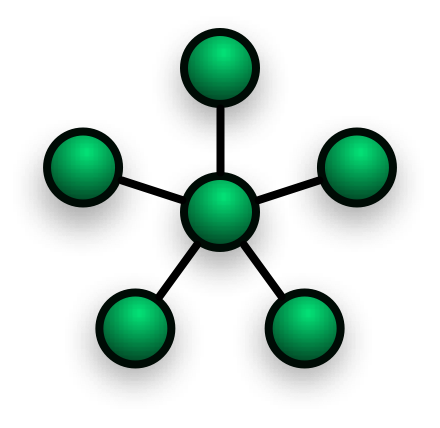
\includegraphics[width=0.49\textwidth]{Bilder/star.png}} 
	\subfloat[Verteiltes Netz \cite{mesh}]{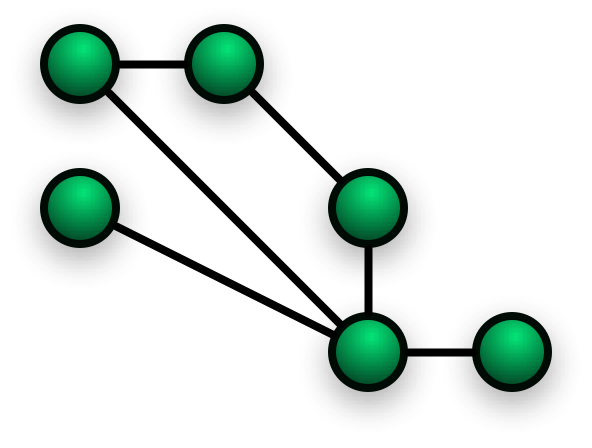
\includegraphics[width=0.49\textwidth]{Bilder/mesh.png}} 
	\caption{Netztopologien} 
	\label{net}
\end{figure}

\noindent Die Blockchain wird �ber ein Peer-to-Peer Netzwerk auf die einzelnen Konten verteilt. Transaktionen innerhalb des Netzwerkes werden als neuer Zustand in der Blockchain gespeichert. Jeder Knoten des Netzwerkes h�lt eine Kopie der Blockchain. \\
Der Begriff der Dezentralisierung bekommt bei der Blockchain eine besondere Bedeutung. Die Dezentralisierung des Netzwerkes sorgt nicht nur f�r Ausfallsicherheit, sondern auch f�r Unabh�ngigkeit. So ist es praktisch unm�glich f�r einen einzelnen die Informationen, die in der Blockchain gespeichert sind zu ver�ndern oder zu zensieren.


\section{Asymmetrische Kryptographie}

Um an einem auf Blockchain basierenden System teilzunehmen, braucht es eine Zugangssoftware. Die Zugangssoftware wird als Wallet bezeichnet und besteht aus einem �ffentlichen und privaten Schl�ssel. Die aus der asymmetrischen Verschl�sselung stammende Technik wird zur Signierung und Adressierung der kryptografischen W�hrung genutzt \cite{stallings}. Zu den bekanntesten asymmetrischen Verschl�sselungsverfahren z�hlen RSA und Diffie-Hellman \cite{RSADH}.
Der �ffentliche Schl�ssel dient als Adresse der Wallet, vergleichbar mit der IBAN-Nummer eines Kontos. Au�erdem kann mit Hilfe des �ffentlichen Schl�ssels, der Kontostand einer Wallet eingesehen werden. Jedoch dient der �ffentliche Schl�ssel als Pseudonym, so dass es nicht m�glich ist, aus ihm die Identit�t des Besitzers zu ermitteln. Dieser �ffentliche Schl�ssel wird bekannt gegeben. F�r Transaktionen ben�tigt man den eigenen privaten Schl�ssel, welcher als Pin der eigenen Wallet fungiert \cite{priv}. Der Absender kombiniert die Nachricht mit seinem privaten Schl�ssel und sendet die signierte Nachricht an die sich aus dem �ffentlichen Schl�ssel ergebende Adresse des Empf�ngers. Mit dem �ffentlichen Schl�ssel des Absenders kann der Empf�nger die signierte Nachricht pr�fen und somit die Authentizit�t der Nachricht verifizieren \cite{badev}. Der Absender der Nachricht kann nicht leugnen, diese signiert zu haben \cite{franco}. Durch die assymmetrische Verschl�sselung kann die Nachricht nicht unbemerkt ver�ndert werden, wodurch deren Integrit�t gew�hrleistet ist \cite{stallings}.

\section{Kryptow�hrungen}
Kryptografische W�hrungen sind eine Art digitales Geld. Im Internet sind diese vielseitig einsetzbar. Zu den gr��ten kryptografischen W�hrungen z�hlen Bitcoin und Ethereum. Mit ihnen k�nnen online Eink�ufe get�tigt oder weltweit innerhalb von k�rzester Zeit W�hrungsbetr�ge versendet werden. Au�erdem werden sie wie die �blichen W�hrungen auf dem W�hrungsmarkt gehandelt und Investoren nutzen sie als Geldanlage genutzt.\\
Der wesentliche Unterschied zwischen gew�hnlichem Geld und Kryptow�hrungen ist die Regulierung sowie die Entstehung des Geldes. Normales Geld wird von einer Zentralbank herausgegeben. Im Vergleich dazu entstehen kryptografische W�hrungen durch Blockchain-Prozesse. \\
Kryptow�hrungen existieren bis auf wenige Ausnahmen nur in der Blockchain. Zu diesen Ausnahmen z�hlt IOTA. �ber eine Wallet erh�lt der Besitzer Zugriff auf seine Kryptow�hrungsanlagen.
Da Digitalw�hrungen nur in der Blockchain existieren, gibt es sie auch nicht in Form von Bargeld im klassischen Sinne. Von einigen W�hrungen, beispielsweise Bitcoin, k�nnen jedoch auch echte M�nzen erworben werden, die den geheimen Code eines einzelnen Bitcoins beinhalten. Allerdings ist hierbei besondere Vorsicht geboten, denn solange der Code noch nicht in die Wallet des Erwerbers �bertragen wurde, ist er anf�llig f�r Angriffe und kann sogar von dem Verk�ufer der M�nze ,,zur�ckgeklaut?? werden, falls dieser den Code noch kennt. \cite{kcur}	

\subsection{Bitcoin}\label{subsec:bitcoin}	

Bitcoin war die erste Kryptow�hrung und ist ma�geblich daf�r verantwortlich, dass der Begriff Blockchain heute so bekannt ist \cite{BITB}. Das Bitcoinsystem ist vollst�ndig und gut in einem Wiki \cite{BC-Wiki} dokumentiert und wird in vielen Arbeiten behandelt oder als Beispiel genutzt. 
Das Bitcoin-Konzept wurde ertsmals 2008 unter dem Pseudonym Satoshi Nakamoto in einem White Paper vorgeschlagen \cite{BC}. Das Einheitenzeichen f�r Bitcoin ist BTC, welches auch oft als Abk�rzung verwendet wird. \\
F�r die Generierung von Bitcoins m�ssen Knoten des Peer-to-Peer Netzwerkes L�sungen zu einem bestimmten, schwer l�sbaren mathematischen Problem finden. In den ersten vier Jahren seit Bestehen des Bitcoin-Netzwerkes wurden 10.500.000 Bitcoin geschaffen. Aller vier Jahre wird dieser Betrag halbiert, sodass sich �ber die Zeit, die Gesamtzahl an Bitcoins 21 Millionen ann�hern wird. Der letzte Block, welcher eine M�nze generiert, wird mit dem jetzigen System etwa im Jahr 2140 erreicht werden. Die derzeitige Gr��e der Bitcoin-Blockchain betr�gt 159 Gigabyte (Stand M�rz 2018) \cite{BCS} . \\
Im Bitcoinsystem wird der Konsensmechanismus Proof-of-Work verwendet. Das Ziel aller Konsensmechanismen ist es, einen Konsens zwischen gegenseitig nicht vertrauensw�rdigen Teilnehmern ohne vertrauensw�rdigen Dritten zu bilden \cite{Block}. Der Grundgedanke von Konsensmechanismen ist es, dass kein Teilnehmer allein den aktuellen Zustandes des Netzwerkes oder eines Teils davon bestimmen kann, es gleichzeitig aber jedem Teilnehmer potenziell m�glich ist den Zustand des Netzwerkes zu ver�ndern. Der jeweilige Konsensmechanismus gibt die Bedingungen vor, die ein Teilnehmer erf�llen muss, um den Zustand des Netzwerkes ver�ndern zu d�rfen. Aus dieser Bedingung wird eine Wahrscheinlichkeit abgeleitet, mit der der Teilnehmer den Zustand tats�chlich ver�ndern wird \cite{BITB}. Im Kontext von Blockchain-Netzwerken besteht die Ver�nderung darin, einen Block anzuh�ngen. Oft wird auch von generieren, erzeugen oder minen eines Blockes gesprochen.
Die Bedingung muss von einem einzelnen Teilnehmer nur schwer zu erbringen, von allen anderen Teilnehmern aber leicht �berpr�fbar sein. Dabei bezieht sich schwer oft auf hohen Rechenaufwand oder eine geringe Wahrscheinlichkeit.\\ 
Bei Proof-of-Work ist die Bedingung der Nachweis einer gewissen Rechenleistung. Dieser Mechanismus wird von Nakamoto mit \textit{one-vote-per-cpu} beschrieben \cite{PoW, BC}.
In Bitcoin ist daf�r in jedem Block eine Zahl enthalten, die so gew�hlt oder besser gefunden werden muss, dass der Hashwert des Blocks kleiner als ein vom Netzwerk vorgegebener Wert ist. F�r jeden Teilnehmer ist der zu berechnende Block unterschiedlich, da die erste Transaktion jedes Blockes eine Transaktion \textit{aus dem Nichts} an den Teilnehmer selbst ist und dort der individuelle �ffentliche Schl�ssel hinterlegt ist. Dadurch und durch die niedrige Warscheinlichkeit die richtige Zahl zu erraten, kann nicht vorhergesagt werden, welcher Teilnehmer den n�chsten g�ltigen Block generiert \cite{PoW}.
Proof-of-Work kann theoretisch einen Teilnehmer mit einer Rechenleistung von \(<50\%\) der Gesamtrechenleistung des Netzwerkes kompensieren. Praktisch wird das Netzwerk aber schon ab \(25\%\) instabil \cite{CC}.

\subsection{Ethereum}

Das Ethereum-System baut auf dem Prinzip der Blockchain auf und dient zur Handhabung von kryptografischen W�hrungen. Dabei wird Ether als interne W�hrung im Ethereum-System verwendet. Im Zusammenhang mit Ethereum sind auch Smart Contracts zu nennen. Dabei handelt es sich um Programme, welche automatisch ausgef�hrt werden, sobald eine festgelegte Summe Ether �berwiesen wurde. Nach der �berweisung startet automatisch die im Vertrag festgelegte Dienstleistung. Smart Contracts werden in der f�r Ethereum entwickelten Programmiersprache Solidity geschrieben. Desweiteren k�nnen dezentralisierte Applikationen auf der Blockchain ausgef�hrt werden, diese werden durch Smart Contracts beschrieben. \\
Ethereum wurde durch die Publikationen \textit{Ethereum: A Next Generation Smart Contract and Decentralized Application Platform} (2013) \cite{ETHW} und \textit{Ethereum Yellow Paper} (2014) \cite{ETHY} beschrieben. Zu den Entwicklern und Mitbegr�ndern des Ethereum-Projekts geh�ren Vitalik Buterin, Gavin Wood und Jeffrey Wilcke. Der Betrieb des Ethereum-Netzwerkes startete Juli 2015 \cite{ETHT}. \\
Als Konsensmechanismus wird Proof-of-Work verwendet, jedoch ist im Entwicklungsplan von Ethereum vorgesehen, dass der Mechanismus auf Proof-of-Stake ver�ndert wird \cite{ETHE}. Proof-of-Work ist sehr rechenintensiv. Proof-of-Stake als Alternative, ist ein deutlich weniger rechenaufwendiger Mechanismus. Die Bedingung ist der Besitz von Anteilen von Token im Netzwerk. Je mehr Anteile ein Teilnehmer besitzt, desto wahrscheinlicher generiert er einen Block \cite{BITB}.

\subsection{Vergleich der exemplarischen Konzepte}

Sowohl Bitcoin als auch Ethereum nutzen die Blockchain als Grundlage ihres Netzwerkes. Bei Bitcoin handelt es sich au�erdem um eine W�hrung, Ethereum nutzt dabei Ether als W�hrung im eigenen System. Bitcoin wurde im Jahr 2009 vorgestellt. Ethereum erstmals im Jahr 2013, allerdings handelt es sich bei Ethereum auch um ein Projekt, welches seit dem st�ndig fortentwickelt wurde. Erkennbar ist es unter anderem, dass der Konsensmechanismus bei Ethereum im Laufe der Entwicklung von Proof-of-Work zu Proof-of-Stake wird. Bitcoin nutzt seit seiner Vorstellung exklusiv Proof-of-Work als Konsensmechanismus.\\
Ein wesentlicher Unterschied ist die Verwendung von Smart Contracts und dezentralisierten Applikationen bei Ethereum. Dadurch wird die Nutzung des Ethereum-Netzwerkes flexibler im Vergleich zum Bitcoin-Netzwerk. Durch Smart Contracts entstehen viele neue Anwendungsfelder f�r die Blockchain-Technologie. Erw�hnenswert sind Lizenzvergabe, Zahlungsabwicklungen oder Vertragsabschl�sse. In den kommenden Jahren werden weitere Gesch�ftsfelder Smart Contracts nutzen. Im Zusammenhang mit Smart Contracts ist der Begriff Token zu nennen. Durch den Ethereum Token Standard, auch ERC20 genannt, ergeben sich f�r Entwickler weitere M�glichkeiten Smart Contracts auf der Ethereum-Blockchain zu nutzen. Durch die st�ndige Weiterentwicklung der Ethereum-Technologie ergeben sich deutlich mehr Anwendungsm�glichkeiten als sie Bitcoin bietet.  
	
\thispagestyle{empty}
\clearpage
\hbox{}\newpage
	
	% Methodik
	\chapter{Methodik}

	Nach Nennung und Erl�uterung wichtiger technischer sowie theoretischer Grundlagen folgen in diesem Kapitel die methodischen Grundlagen, mit der diese Arbeit erstellt wird. Hierbei wird im ersten Abschnitt auf Interviews eingegangen, welche im weiteren Verlauf gef�hrt werden, um aus Kundensicht den ideal Prototyp einer Ethereum-basierten App herzustellen. Der zweite Abschnitt behandelt das Thema \textit{Tello}, welches genutzt wird, um innerhalb eines Teams die �bersicht �ber das Projekt zu wahren. Die Grundlagen �ber Machbarkeitsstudien sowie Risikoanalysen bilden das Ende des Kapitels.
	
	\section{Methodische Grundlagen der Interviews}
		
		Um aus Herstellersicht zu erfahren, inwiefern sich ein Produkt f�r ein Kunden eignet und welche Schwerpunkte bei der Entwicklung gelegt werden m�ssen, ist es n�tig Anforderungen und W�nsche zu ermitteln. Dies kann auf mehreren Wegen geschehen, beispielsweise in Form von printbasierten Medien. Der Nachteil hierbei ist allerdings, dass vorgedruckte Fragen oftmals zu ungenau auf kundenspezifische Anliegen eingehen. Eine aufw�ndigere, allerdings deutlich pers�nlichere und daher kunden�here Form der Befragung ist das Interview. Hierbei stehen Hersteller sowie Kunde im direkten Kontakt. Somit ist es m�glich, innerhalb eines Gespr�chs detailliert auf konkrete W�nsche und Vorstellungen des Kunden einzugehen und etwaige Problematiken zu diskutieren. Ein weiterer Vorteil ist die Beschreibung der Arbeitsabl�ufe seitens des Herstellers, was zu mehr Verst�ndnis durch den Kunden f�hrt und so die Arbeit in der Regel f�r alle Parteien erleichtert. Ein Nachteil des Interviews ist der erh�hte Zeit- und Personenaufwand. In diesem Abschnitt werden die Rahmenbedingungen f�r das Interview gelegt, welches im weiteren Verlauf gef�hrt wird, um die Anforderungen an einen m�glichen Prototypen festzustellen.\\
		
		Die Vorbereitung f�r ein Interview betreffen beide Seiten, wobei prim�r der Hersteller betroffen ist. Dieser hat die Aufgabe, spezifische Fragen zu stellen und m�glichst viele W�nsche des Kunden zu erfassen und konkrete Anforderungen daraus abzuleiten. Je detaillierter die daraus resultierenden Antworten sind, desto spezifischer kann der Hersteller im weiteren Verlauf sein Produkt auf die W�nsche des Kunden anpassen. Der Hersteller hat die Aufgabe, das richtige Personal f�r ein Interview bereitzustellen. Dieses Team besteht im Idealfall aus Experten, welche sich bereits mit der Thematik, in diesem Falle Ethereum und App Entwicklung, auskennen und den Kunden im Laufe des Interviews beraten k�nnen. Aus Kundensicht ist es n�tig, im Voraus Anforderungen und konkrete Vorstellungen beschreiben zu k�nnen. W�hrend des Interviews ist es beiden Seiten m�glich, den Gespr�chsverlauf dynamisch zu beeinflussen und so bisher nicht erkannte Probleme anzusprechen. Das Interview sollte gut dokumentiert werden, um eine sp�tere Auswertung f�r den Hersteller zu erm�glichen. Eine abschlie�ende Zusammenfassung der wichtigsten Punkte, insbesondere noch ungekl�rter Fragen, helfen sowohl Kunde als auch Dienstanbieter bei der Entwicklung. Es ist daher m�glich, neben dem initialen Interview auch weitere pers�nliche Gespr�che zu f�hren, um das Produkt bestm�glich an den Kunden anzupassen. Um die wichtigsten Aspekte beim Einf�hren einer Software im Gastronomiebereich zu etablieren, werden Experteninterviews durchgef�hrt. Es werden Gastronomien im umliegenden Bereich interviewt. Daber wird eine semigeleitete Interviewform gew�hlt, um m�glichst individuelle Informationen, wie zum Beispiel Wissensstand �ber Blockchain oder dem tats�chlichen Einsatz des Szenarios in dem Betrieb. Diese Informationen werden anschlie�end ausgewertet, um eine Ausblick f�r weitere Untersuchungen zu schaffen. Auf Herstellerseite ist es von Nutzen, besonders f�r kleinere Projekte wie die in dieser Arbeit erstellte Ethereum App, mithilfe von spezieller Software Anregungen des Kunden festzuhalten und den aktuellen Fortschritt des Produkts festzuhalten. Ein Beispiel f�r diese Software ist \texttt{Tello}, welche im n�chsten Abschnitt n�her erl�utert wird.
		
	\section{Projektmanagement-Werkzeug \textit{Trello}}	
	
		Aufgrund des limitierten Projektumfangs sowie der Notwendigkeit zur Einarbeitung von dynamischen �nderungsanfragen wurde im Rahmen der Projekt- und Dokumententwicklung ein agiler Projektmanagement-Prozess realisiert, welcher intern auf einer Kombination der klassischen Vorgehensmodelle \textit{Scrum} und \textit{Kanban} basiert \textcolor{red}{[11]}. %QUelle: http://www.agiles-projektmanagement.info/scrum-und-kanban-im-vergleich/ 
		Die Projektbearbeitung zeichnet sich bei Verwendung dieser agilen Modelle insbesondere durch ein iteratives Vorgehen in enger Abstimmung mit dem Auftraggeber aus, sodass die phasenweise produzierten Produkt-Artefakte kontinuierlich verfeinert werden k�nnen. Die Realisierung von zentralen Teilkomponenten des finalen Produkts wird dabei innerhalb sogenannter \textit{Sprints} aggregiert, welche eine zeitlich limitiert Phase mit dediziertem Implementierungsschwerpunkt repr�sentieren.
		
		Zur Koordination des konkreten Produktionsprozesses wurde bei Projektinitialisierung die Verwendung eines zentralen Kanban-Boards beschlossen, welches prim�r als tabellarisches Visualisierungselement der projektinternen Teilaufgaben fungieren sollte. Auf diese Weise k�nnen die anfallenden Aufgaben explizit ausgew�hlten Projektmitgliedern zugewiesen werden, welche die jeweiligen Teilaufgaben auf Basis des internen Fortschritts in verschiedene Entwicklungs-Stufen klassifizieren k�nnen. 
		
		Aufgrund der limitierten Ressourcenlage sowie des hohen Zusatzaufwandes, den der lokale Betrieb einer dedizierten Software-L�sung wie \textit{Atlassian Jira} oder \textit{OpenProject} induziert, fiel die Entscheidung auf die Nutzung des kostenfreien Web-Anbieters \textit{Trello}.
		Innerhalb der Trello-Umgebung wird ein dynamisch rekonfigurierbares Kanban-Board bereitgestellt, dessen Inhalte interaktiv in der Browser-Umgebung administriert werden k�nnen. Die Struktur kann hierbei individuell an die individuellen Projektanforderungen angepasst werden; aufgrund der Einfachheit in der Bedienung sowie der M�glichkeit zur kollaborativen Nutzung mit weiteren Mitgliedern hebt sich das Tool hierbei von vergleichbaren Anbietern ab \textcolor{red}{[11]}.
		%Quelle:https://t3n.de/news/to-do-tools-test-451433/
		Trello fasst die Projektmitglieder zu einem Team zusammen, innerhalb dessen unter Verwendung von grafischen Visualisierungshilfen das Anlegen und die Bearbeitung von Teilaufgaben (in der Trello-Terminologie als \textit{Karten} bezeichnet) koordiniert werden kann. Die Aufgaben k�nnen dabei durch individuelle Markierungen gezielt an einzelne Teammitglieder delegiert werden, sodass die Zust�ndigkeiten innerhalb des Projekts stets klar gekl�rt sind. Weiterhin k�nnen im Kontext der Aufgaben-Spezifikation integrierte Zusatzfunktionalit�ten wie Fristen und Checklisten genutzt werden, sodass beispielsweise eine schrittweise Realisierung einzelner Teilaufgaben erm�glicht wird.
		
		Strukturell wurde das Kanban-Board f�r die Anwendungs- und Dokumententwicklung in f�nf Spalten separiert, wobei die drei elementaren Entwicklungs-Stufen der Aufgaben durch ein initiales Kommunikationselement und eine �bersicht der aktuellen Sprint-Ziele eingeschlossen werden. Diese grundlegende Konfiguration der Trello-Umgebung nach Abschluss der ersten Initialisierung ist exemplarisch in Abbildung REF unten dargestellt.\\
		
		\begin{figure}[h] 
			\centering
			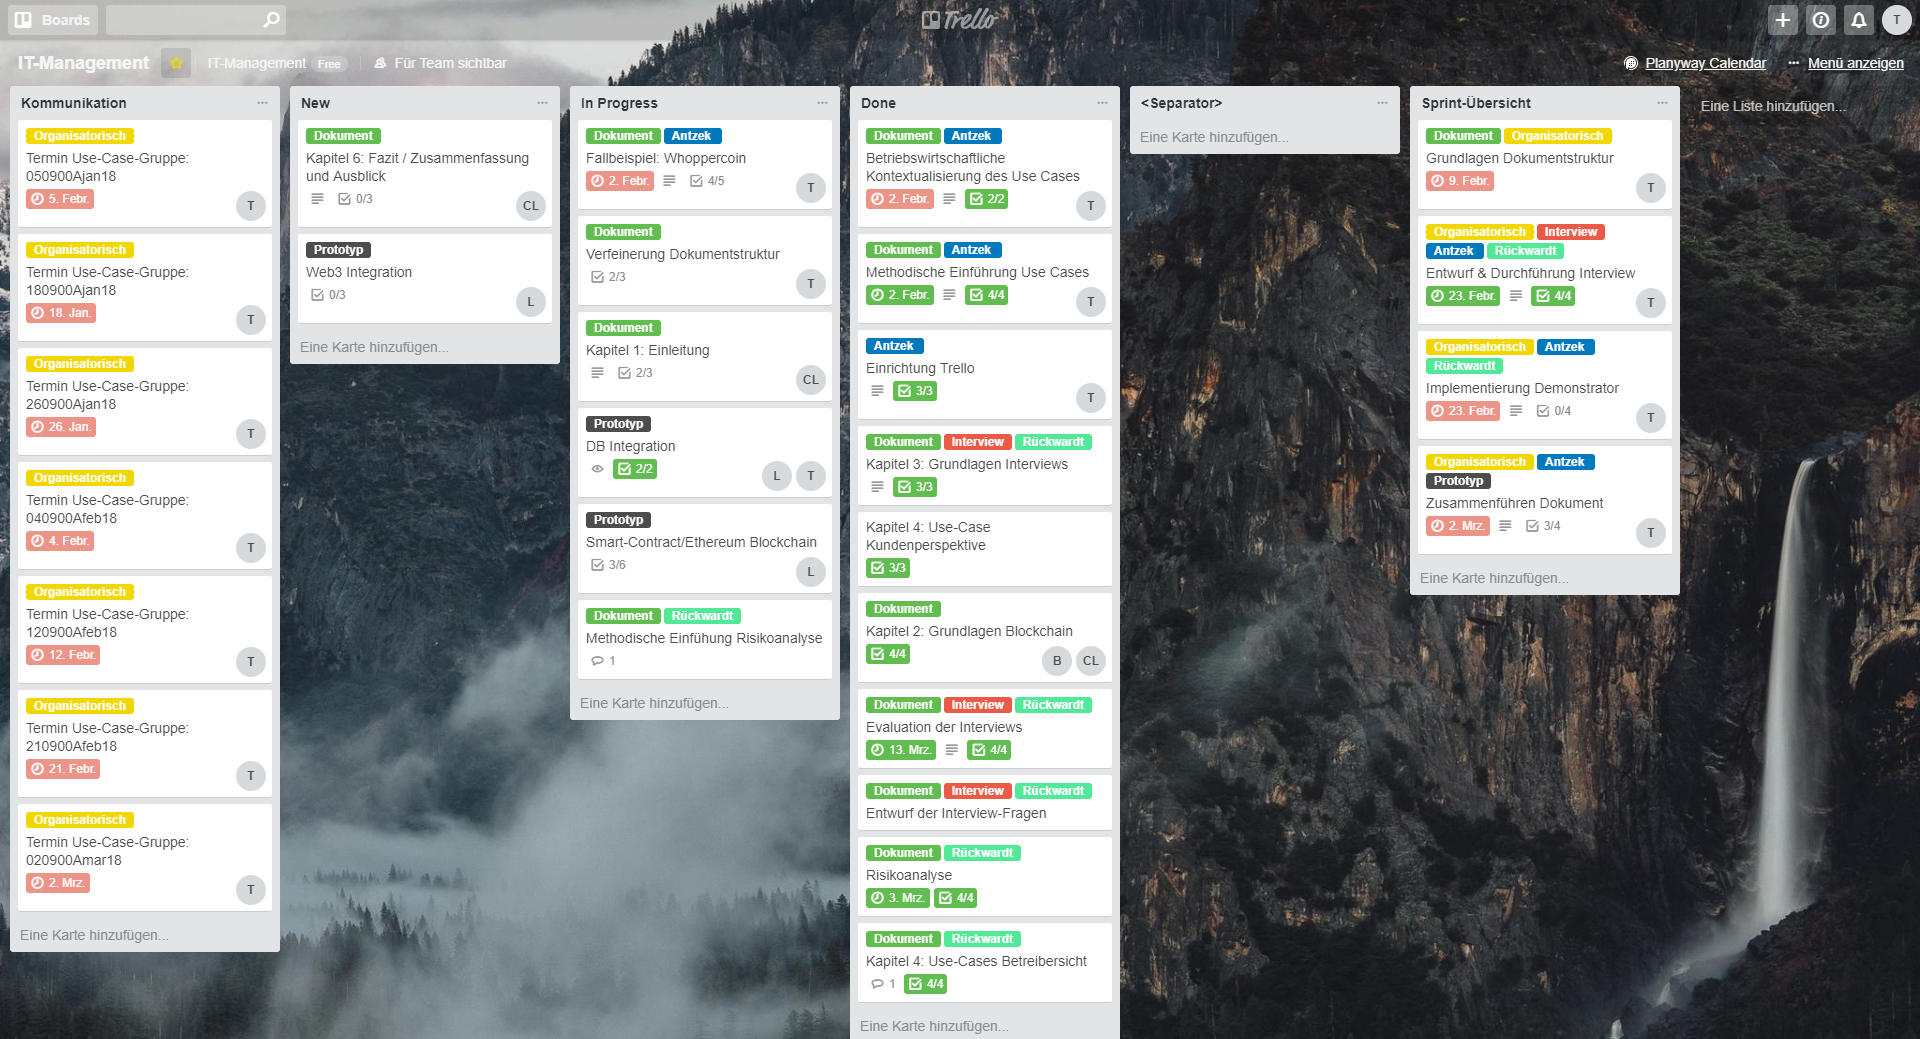
\includegraphics[width=0.9\textwidth]{Bilder/trello_0.png}
			\caption[\textcolor{red}{TODO}]{\textcolor{red}{TODO}}
			\label{fig:trello_0}
		\end{figure}
		
		Die drei zentral angeordneten Spalten \textit{New}, \textit{On Progress} und \textit{Done} repr�sentieren die angesprochenen Fortschrittsstufen der individuellen Teilaufgaben. Initial werden neue Aufgaben innerhalb der Spalte \textit{New} deklariert und einem Team-Mitglied zugewiesen, welches vor Beginn der Bearbeitung die internen Parameter und Schnittstellen exakt spezifiziert. Sobald die Arbeit an einer Teilaufgabe begonnen wird, wird das korrespondierende Karten-Element f�r alle sichtbar in die Spalte \textit{In Progress} verschoben. Auf diese Weise verf�gen alle Teammitglieder �ber eine aktuelle �bersicht des Bearbeitungsstatus; dies erm�glicht bei Konflikten oder partiellen �berlappungen eine vereinfachte Koordination der beteiligten Akteure. Nach Abschluss der Bearbeitung erfolgt die Verschiebung der Karte in die Spalte \textit{Done}, wobei anhand der internen Checklisten des Karten-Elements die Vollst�ndigkeit der Bearbeitung validiert werden kann. Die Resultate werden final durch einen Vertreter der Gruppenleitung �berpr�ft, sodass eine konfliktfreie Integration der Teilresultate in den globalen Bearbeitungsstand garantiert werden kann. Die Akzeptanz einer Teilaufgabe durch die Gruppenf�hrung wurde projektintern durch Aktivieren der Frist-Checkbox signalisiert, welche die Karte f�r den weiteren Projektverlauf als inaktiv markiert (vergleiche Abbildung XX unten).
		
		\begin{figure}[h] 
			\centering
			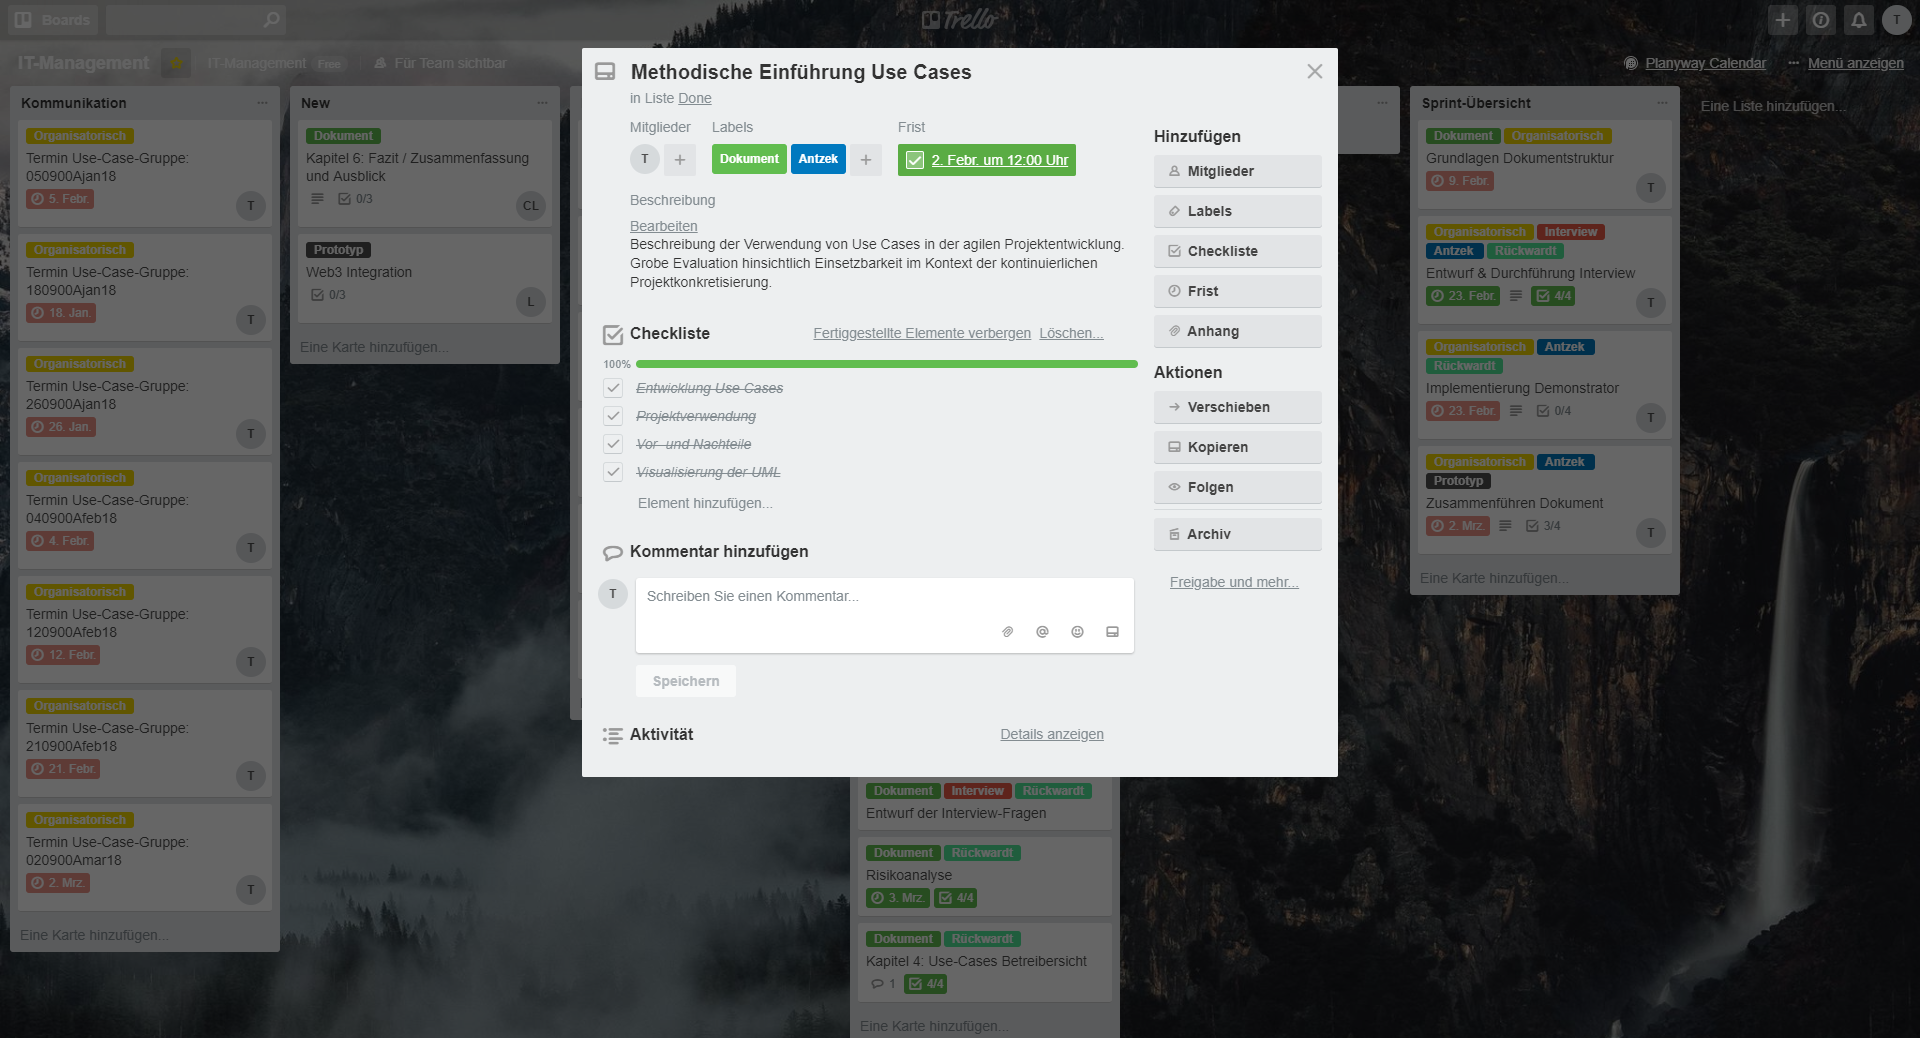
\includegraphics[width=0.9\textwidth]{Bilder/trello_1.png}
			\caption[\textcolor{red}{TODO}]{\textcolor{red}{TODO}}
			\label{fig:trello_1}
		\end{figure}
		
		
		Durch die Verwendung einer internen Projektmanagement-Anwendung konnten im Projektverlauf �berlappungen und Kollisionen in der Aufgabenbearbeitung weitestgehend vermieden werden. Die Wahl eines agilen Konzeptes erm�glichte dabei die Anpassung an die individuellen Projektparameter, ohne jedoch �berm��igen Verwaltungsaufwand zu induzieren.
		
	\section{Risikoanalyse}	
	
		Nach der Betrachtung der UseCases erfolgt eine kurze Risikoanalyse des Produktes \cite{Stelzer2002}. Im Rahmen des Projektmanagements bedeuten Risiken in erster Linie Unsicherheiten, die sich negativ auf den Projektverlauf auswirken k�nnen. Definiert man das Risiko rein mathematisch, handelt es sich um einen Zustand, der eintreffen kann oder nicht. In Betrachtung des Projektmanagements sind Risiken jedoch reale und virtuelle Ereignisse, die einen realen Schaden am Projekt hervorrufen k�nnen. Der Eintritt eines Risikos zieht also immer negative Auswirkungen mit sich. Dazu z�hlen folgende drei Faktoren, die alle drei betroffen sein k�nnen, aber nicht zwingend m�ssen: Zeit, Kostend und Qualit�t. Die Risikoanalyse im Rahmen dieses Projektes hat zum Ziel, Risiken im fortlaufenden Projekt zu erkennen, zu analysieren und die Wahrscheinlichkeit des Eintreffens der Risiken mit den daraus resultierenden Folgen zu ermitteln. Als weiteres Ziel schafft die Risikoanalyse die M�glichkeit einen Entscheidungsprozess zu optimieren und zu objektivieren. Der erste Schritt zur Durchf�hrung einer Risikoanalyse im Rahmen des Projektmanagements besteht darin Risiken zu erkennen. Bei der Ermittlung der Risiken ist zu beachten, dass zwischen verschiedenen Risiken (externe Risiken, interne Risiken, planerische Risiken, kaufm�nnische-, fachliche- und Umfeld-Risiken) unterschieden wird. Die nachfolgenden Schritte dienen der Risiko�bersicht, der Befragung von Projektbeteiligten, dem Studium der Projektunterlagen und der Analyse im laufenden Betrieb. Das Wegfallen und Entstehen von Risiken begleitet das gesamte Projekt �ber die gesamte Laufzeit. Dies macht eine erg�nzende Analyse der Risiken, ihrer Wahrscheinlichkeiten und Folgen unabdingbar. 
	
	\chapter{\label{chap:4szenario}Szenariodefinition}
	
	Auf Basis der innerhalb des vorhergehenden Kapitels formulierten technischen sowie methodischen Kontextualisierung werden im Rahmen dieses Abschnittes multiperspektivisch exemplarische Nutzungsszenarien der Blockchain-Technologie diskutiert und final hinsichtlich ihrer Realisierbarkeit in produktiven Umgebungen des Gastronomie-Sektors evaluiert. Aufbauend auf einer initialen Definition der betriebswirtschaftlichen Terminologie werden dabei aus den Erfahrungen der \textit{Whoppercoin}-Implementierung elementare Use-Cases zur Entwicklung neuer Anwendungskonzepte f�r den gastronomischen Bereich extrahiert.
	
	
	\section{Betriebswirtschaftliche Kontextualisierung}
		
		Innerhalb der letzten Jahre ist sowohl f�r den privaten als auch f�r den industriellen Sektor eine kontinuierliche Intensivierung der Digitalisierungsanstrengungen zu konstatieren. Insbesondere im gewerblichen Kontext sind kontinuierliche Optimierungen der digitalen Infrastruktur zu einer wesentlichen Voraussetzung f�r wirtschaftlichen Erfolg und internationale Konkurrenzf�higkeit geworden; unterst�tzt durch die  permanente technologische Entwicklung sind innerhalb produktiver Unternehmensumgebungen automatisierte Datenverarbeitungs-Prozesse sowie digitalisierte Kommunikationsstrukturen heute weitestgehend omnipr�sent. Gem�� der im Jahre 2015 publizierten Studie \textit{d!conomy - Die n�chste Stufe der Digitalisierung} des Bundesverbands Informationswirtschaft, Telekommunikation und neue Medien e. V. (Bitkom) bewertet die Majorit�t der Unternehmen in Deutschland mit 86\% (im industriellen Sektor sogar 93\%) Zustimmung die durch Digitalisierung induzierten Transformationsprozesse als positiv \textcolor{red}{[11]}; %Quelle: https://t3n.de/news/digitalisierung-studie-bitkom-cebit-599910/
		auf Basis dieser Stimmungslage pr�diziert das Marktforschungsinstitut \textit{Kantar Taylor Nelson Sofres} (Kantar TNS) 2017 die in Abbildung \ref{fig:digit} visualisierte, signifikante Inkrementierung des innerdeutschen Digitalisierungsgrades aller Branchenzweige bis zum Jahr 2022 \textcolor{red}{[11]}.%Quelle: https://www.tns-infratest.com/wissensforum/studien/mrwd.asp
		
		\begin{figure}[h] 
			\centering
			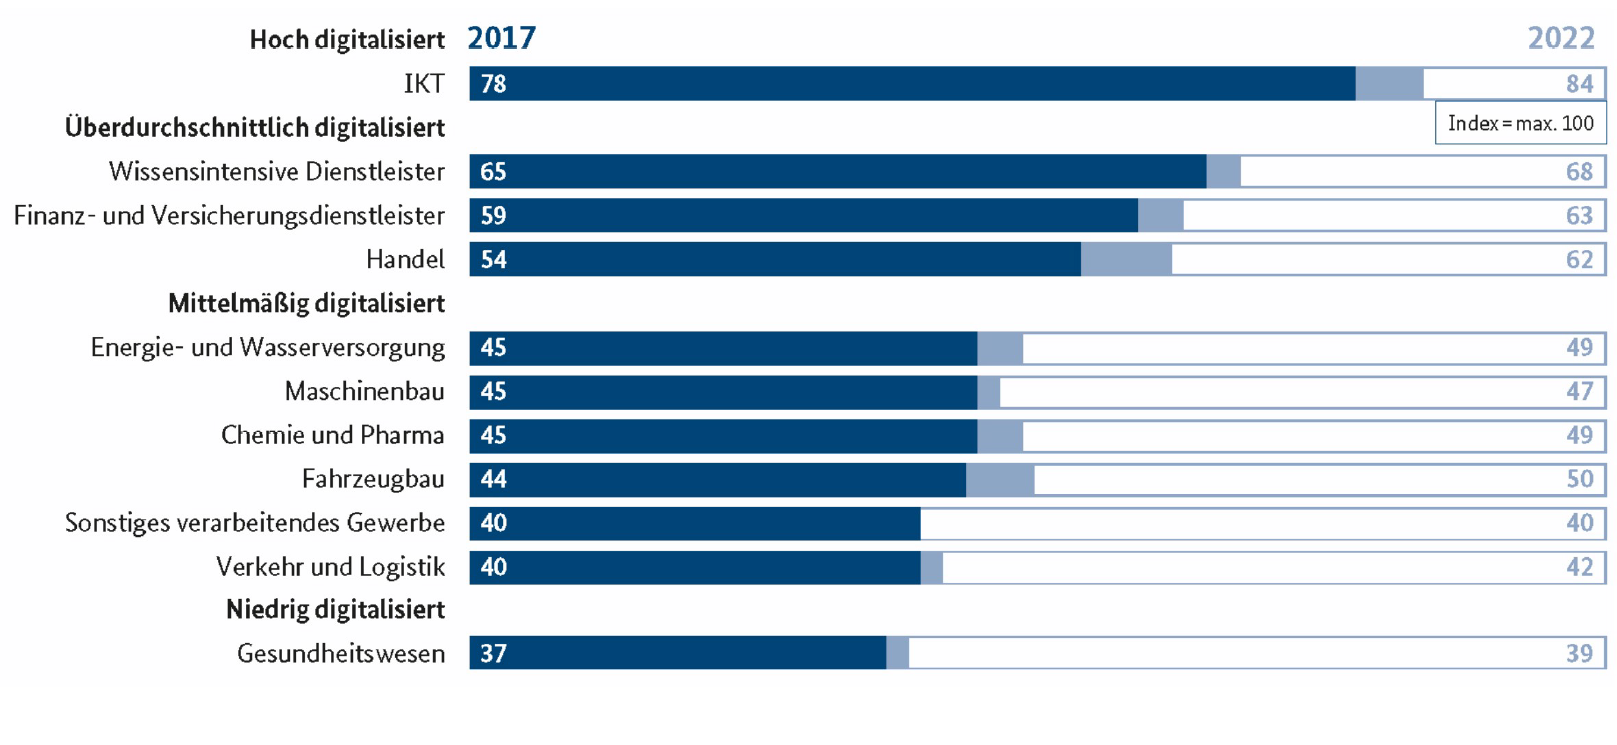
\includegraphics[width=0.82\textwidth]{Bilder/digittrend-mini.png}
			\caption[Repr�sentative Unternehmensumfrage zur Digitalisierung 2017]{Repr�sentative Unternehmensumfrage \mbox{zur Digitalisierung 2017 (nach \textcolor{red}{[11]})}}%Quelle: https://www.tns-infratest.com/wissensforum/studien/mrwd.asp
			\label{fig:digit}
		\end{figure}		
		
		\noindent Prim�r wird die sukzessive Einf�hrung einer digitalisierten Infrastruktur f�r die Unternehmen dabei durch die potentielle Effizienzmaximierung in klassischen Sektoren wie Produktion, Logistik und Ein- und Verkauf motiviert \textcolor{red}{[11]}; sekund�re Aspekte werden durch die Optimierung interner Prozesssteuerungs- und Controlling-Elemente sowie die Verbesserung der Kundeninteraktion repr�sentiert, deren Priorisierung in Abh�ngigkeit vom individuellen Unternehmensschwerpunkt markant divergieren kann \textcolor{red}{[11]}.\\
		% Quelle: https://www.pwc.de/de/digitale-transformation/digital-factories-2020-shaping-the-future-of-manufacturing.pdf
		% Quelle: http://news.aucotec.com/factory-future-digital-13-statistics-know-heading-2018/
		\noindent Die moderne Interpretation des Terminus \textit{Digitalisierung} erweitert den urspr�nglichen Optimierungsgedanken um einen weiteren Aspekt, welcher die IT in der Rolle eines Prozess-\textit{Enablers} darstellt. Auf Basis der durch Informationstechnologie offerierten Funktionalit�t k�nnen dabei fundamental neue Gesch�ftsmodelle, Produkte und Dienstleistungen generiert werden; IT-basierte Innovationen fungieren somit nicht l�nger nur zur Optimierung bereits bestehender Prozessstrukturen, sondern k�nnen in ihrer Rolle als unmittelbare Voraussetzung (\textit{Enabler}) die radikale Reorganisation von Prozessen und Wertsch�pfungsketten induzieren \textcolor{red}{[11]}. %Quelle: https://link.springer.com/content/pdf/10.1007/978-3-658-10640-9_2.pdfg 
		%Die heutige Digitalisierung geht jedoch einen wesentlichen Schritt weiter: Unternehmen
		%entwickeln heute auf der Basis von Informationstechnologien fundamental neue Gesch�ftsmodelle,
		%Produkte und Dienstleistungen. IT-Innovationen dienen nicht nur der
		%Unterst�tzung, sondern der radikalen Neugestaltung von Prozessen und Wertsch�pfungsketten.
		%So entstehen neue Wertsch�pfungsnetze und die Strukturen und Kr�fteverh�ltnisse
		%ganzer Branchen ver�ndern sich; traditionelle Branchengrenzen verschwimmen. IT-induzierte Innovationen fungieren in diesem Kontext als Enabler f�r zentrale %Unternehmensprozesse
		%offeriert nicht nur Optimierung bestehender Prozesse wie Logistik o�, sondern offeriert oftmals Grundlage zur Entstehung innovativer L�sungsans�tze.
		\mbox{Konzeptionell} k�nnen die identifizierten IT-Innovationsans�tze nach dem Kriterium des initialen Innovationsimpulses kategorisiert werden, wobei grobgranular zwischen technologieinitiiertem Transformationsdruck (\textit{technology push}) und dem externem Marktsog (\textit{market pull}) differenziert wird.
		Im Kontext des \textit{technology push} wird das Innovationselement durch Resultate technologischer Entwicklung repr�sentiert, welche potentiell die Generierung bisher nicht existenter Marktsegmente induzieren und somit hohes Ertragspotenzial bieten. Die kontr�re Strategie des \textit{market pull} realisiert hingegen die  Extraktion von potentiellen Kundenbed�rfnissen aus der dynamischen Analyse bereits existierender Marktanteile, auf deren Grundlage technische Optimierungsans�tze f�r Produkte, Dienste und Anwendungen abgeleitet werden \textcolor{red}{[11,12]}.
		%Quelle: https://www.uzh.ch/iou/orga/ssl-dir/wiki/uploads/Main/TIM_HS07_Teil_IV.pdf		
		%Skript IT-Governance - Einf�hrung - Dipl.-Wirt.-Inf.	Sebastian	D�nnart	
		Im konkreten Unternehmenskontext ist unter Ber�cksichtigung der individuellen Schwerpunkte jedoch meist eine Form der hybriden Implementierung zu pr�ferieren, um die individuellen Defizite der Konzepte durch selektive Rekombination ausgew�hlter Faktoren zu eliminieren. Die strikt isolierte Realisierung einer Innovationsstragie kann mitunter in der Gef�hrdung der Marktposition resultieren; so besteht bei \textit{technology push} das Risiko zur Entwicklung eines Produktes ohne Markt, w�hrend im Kontext des \textit{market pull} der Fokus auf kontinuierliche Minimaloptimierungen des Ursprungsprodukts (auch als \textit{facelift} bezeichnet) die Realisierung tats�chlicher Innovationen obstruieren kann \textcolor{red}{[11]}. %Quelle: http://www.b4development.com/archives/904
		Ausgehend von dem individuellem Leistungs- und Wachstumspotenzial eines Unternehmens ist dabei die Konzeption einer adaptiven Selektionsstrategie elementar wichtig, um unter Ber�cksichtigung von dynamischen Marktumgebungen und potentiell tempor�ren Tendenzen erfolgversprechende Produkt- und Dienstleistungsparameter zu definieren.\\
		%- Grafiken IT-Management
		%BCG Matrix
		%	aufgrund aktueller Trend hohes potentielles Marktwachstum, Investition lohnt;
		%	wie in BCG-Matrix (http://www.manager-wiki.com/images/stories/Strategieentwicklung/bcg\%20normstrategien.jpg) visualisiert, Question Marks
		%	jetzt zu Stars transformierbar durch adaptive Selektionsstrategie.
		Ein kritisches Element in der unternehmensinternen Digitalisierungsstrategie wird durch die als \textit{Business-IT-Alignment} bezeichnete, strategische  Synchronisation von produktiver Unternehmenskomponente und den korrespondierenden IT-Abteilungen repr�sentiert. Nur die absolute Kongruenz in der Zielspezifikation von Unternehmensleitung und IT-Administration erlaubt die Generierung der reziproken Synergieeffekte, welche den Transfer der IT-Innovationen in den produktiven Kontext erm�glichen und somit final in der Stabilisierung und weiteren Expansion des individuellen Marktanteils resultieren \textcolor{red}{[11]}.
		%Quelle: https://www.uni-bamberg.de/isdl/transfer/it-business-alignment/
		
		
	\section{Fallbeispiel: Whoppercoin Burger King}	
	
		%TODO 
		Wie bereits im Rahmen der vorangehenden Ausf�hrungen dargelegt, kann die Entwicklung neuer \textit{Enabler}-Technologien signifikante �nderungen in verschiedensten Gesch�ftsbereiche induzieren. Aufgrund der weitestgehend universellen Einsetzbarkeit als dezentralisiertes Transaktionssystem werden aktuell das in Abschnitt \ref{subsec:bitcoin} pr�sentierte Blockchain-Konzept sowie die korrespondierenden Erweiterungen als potentielle Innovationselemente f�r den Betrieb zahlreicher Branchenbereiche gehandelt. 
		Der Entstehungsprozess der Blockchain-Technologie wird dabei durch eine Kombination der Entwicklungsstrategien \textit{business pull} und \textit{technology push} repr�sentiert. Als eines der initialen Motive zur Realisierung der Blockchain-Implementierungen wird mitunter der marktseitige Bedarf nach einem digitalen, dezentralisierten W�hrungssystem, sodass im Entstehungskontext von Bitcoin und vergleichbaren Blockchain-Implementierungen eine grundlegende Korrelation mit dem Konzept des \textit{business pull} konstatiert werden kann. Im Rahmen der kontinuierlichen Forschungsintensivierung innerhalb dieses Themenkontextes konnten jedoch sukzessive auch innovative Einsatzszenarien durch die entwickelten Technologien induziert werden, welche insbesondere unter Verwendung generischer Plattformen wie Ethereum zunehmend diversifizierte Funktionalit�t offerieren k�nnen.\\
		Die hierdurch generierte, mediale Pr�senz der Blockchain-Thematik visualisiert das aktuelle Expansionspotential dieses Marktsegments, welches von Analysten der Banken- und Finanzbranche zunehmend als Investitionsfeld der Zukunft propagiert wird \textcolor{red}{[11,11]}. 
		%Quelle: http://www.businessinsider.de/blockchain-in-banking-2018-1-14?r=US&IR=T, https://www.shapingtomorrow.com/home/alert/665529-Future-of--Blockchain
		Die Partizipation in der Blockchain-Forschung sowie die Adaption der entwickelten Technologiel�sungen in produktiven Unternehmensteilen erm�glichen den Unternehmen dabei die Manifestation oder Expansion ihrer Positionierung innerhalb des korrespondierenden Marktsegmentes, wobei die reinen Optimierungsaspekte der offerierten Funktionalit�t durch das marketing-technische Instrumentalisierungspotential der weitestgehend positiven Blockchain-Reputation unterst�tzt werden. Exemplarisch seien an dieser Stelle die signifikanten Kursanstiege der Unternehmen \textit{Kodak} und \textit{Long Island Ice Tea} in Reaktion auf deren partielle Blockchain-Einf�hrung zu Jahresbeginn 2018 referenziert \textcolor{red}{[11,12]}.\\ %Quelle: %https://www.heise.de/newsticker/meldung/Aktienkurs-verdoppelt-Kodak-setzt-jetzt-auch-auf-Blockchain-und-Kryptogeld-3938074.html
		%http://www.handelsblatt.com/finanzen/maerkte/devisen-rohstoffe/long-island-iced-tea-500-prozent-plus-durch-namensaenderung-in-long-blockchain/20767496.html
		\noindent Analog hierzu k�ndigte im August 2017 auch die US-amerikanische Schnellrestaurantkette \textit{Burger King} f�r die nahe Zukunft die Akzeptanz von Bitcoin-Zahlungen sowie die Implementierung einer eigenen Cryptow�hrung, intern als \textit{Whoppercoin} bezeichnet, an. 
		% Quelle:https://www.cnbc.com/2017/08/28/burger-king-russia-cryptocurrency-whoppercoin.html
		In der aktuellen Konfiguration repr�sentiert die vorerst auf russische Filialen limitierte Technologie die Testphase einer dedizierten Kundenbindungsma�nahme, welche die Auszahlung der digitalen W�hrung �quivalent zu bekannten Treuepunkte-Konzepten realisiert. Technologisch basiert die Einf�hrung dabei auf der Instrumentalisierung einer bereits existierenden Blockchain-Infrastruktur, welche durch die Handelsplattform des externen Drittanbieters \textit{Waves Go.} offeriert wird \textcolor{red}{[11]}. % https://www.derstandard.de/story/2000063303882/whoppercoin-burger-king-bringt-eigene-kryptowaehrung-an-den-start
		Durch diese Form der Kooperation kann die Generierung potentieller Synergieeffekte zwischen den Unternehmenen forciert werden; unter Minimierung des individuellen Risikos f�r die beteiligten Instanzen bei gleichzeitiger Partizipation an potentiellen Gewinnen kann eine vorsichtige Evaluation dieses Marktsegmentes bei weitestgehender Gef�hrdungsminimierung f�r die individuelle Kerngesch�fte realisiert werden. Dieses Vorgehen illustriert die ubiquit�re Ambivalenz aus grundlegender Skepsis gegen�ber dieser potentiell revolution�ren Datenverwaltungs-Technologie und dem individuellen Innoviationswillen der Unternehmen bei der Einf�hrung dieser Technologien. Wesentliche Parameter des vorgestellten \textit{Whoppercoin}-Konzeptes werden dabei jedoch von W�hrungsspezialisten und Sicherheitsanalysten als kritisch rezensiert; insbesondere die namentliche Bindung der digitalen W�hrung an ein dediziertes Unternehmen k�nnte die Universalit�t m�glicher Einsatzszenarien limitieren, da die Akzeptanz der \textit{Whoppercoin}-W�hrung durch direkte Konkurrenten wie \textit{McDonald's} als unwahrscheinlich einzustufen ist \textcolor{red}{[11]}.	
		Weiterhin kann eine enge Namenskorrelation zwischen Unternehmen und W�hrung final in kritischen Imagesch�den f�r den Betreiber resultieren, wenn Kontributionen des entsprechenden W�hrungsderivats zu Transaktionen im Kontext strafrechtlich relevanter T�tigkeiten identifiziert und publiziert werden \textcolor{red}{[11]}.
		%Quelle: http://www.businessinsider.de/whoppercoin-burger-king-hat-jetzt-eine-eigene-krypto-waehrung-2017-8
		Aktuell pr�sentiert sich Burger King mit dem vorgestellten Konzept als branchen�bergreifender Vorreiter, wobei das Nachziehen weiterer Unternehmen zeitnah erwartet werden kann. \\
		
	\section{Use Cases im Gastronomie-Kontext}
	
		Aufbauend auf den theoretischen Erkenntnissen der vorherigen Abschnitte soll im Rahmen dieses Dokumentes eine exemplarische Demonstrator-Implementierung f�r die Blockchain-Anwendung im gastronomischen Kontext konzipiert und realisiert werden. Hierzu werden initial die zentralen Anwendungsf�lle aus Perspektive der beteiligten Aktoren identifiziert, wobei auch potentielle Vor- und Nachteile der Blockchain-Technologie illustriert werden.\\
		Die manuelle Spezifikation von \textit{Use Cases} (deutsch: Anwendungsf�lle), deren konzeptionelle Grundlage 1987 durch Ivar Jacobson publiziert wurde, erm�glicht die Modellierung und Dokumentation der systeminh�renten Funktionalit�t bereits existierender oder geplanter Produktkomponenten, indem von konkreten Implementierungsparametern abstrahiert m�gliche Interaktionsszenarien zwischen Aktoren und dem Zielsystem definiert werden.
		Die Aktoren k�nnen hierbei sowohl durch reale Personen als auch durch abstrakte Rollen oder externe Systeme repr�sentiert werden, welche die zur Erreichung eines pr�zise spezifizierten Zieles erforderlichen Interaktionsmuster mit dem Zielsystem simulieren. Die konkreten Attribute des korrespondierenden Use Cases illustrieren dabei neben der Aktor-Komponente auch die extern erkennbaren Reaktionen des Systems, um final m�gliche Konnektionen zwischen Aktorverhalten und systeminternen Abl�ufen identifizieren zu k�nnen. Abl�ufe werden in diesem Kontext als Folge von individuellen Aktionen definiert, welche final in Erfolg oder Fehlschlag des angestrebten Systemprozesses resultieren; hierbei ist zus�tzlich die hierarchische Komposition einzelner Ablaufbeschreibungen m�glich, um die funktionelle Systembeschreibung sukzessive in konkrete Implementierungsparameter zu transformieren. Da eine Visualisierung von komplexen Systemprozessen in Form der oftmals grafisch illustrierten Aktionsfolgen die Kommunikation im Rahmen einer Projektentwicklung signifikant verbessern kann, wird das Konzept der Use Cases h�ufig im Bereich der Produktentwicklung und Kundenabstimmung eingesetzt \textcolor{red}{[11]}.\nopagebreak\\%Quelle:https://www.microtool.de/was-sind-use-cases/
		\noindent Die prim�re Funktion von Use Cases wird durch die initiale Konkretisierung der im Rahmen eines Projektes zu realisierenden Produktfunktionalit�t repr�sentiert, deren detaillierte Beschreibung die Basis f�r die Erstellung eines stringenten Entwicklungskonzeptes darstellt. Um sp�tere Restrukturierungen dieses Konzeptes und damit verbundene Verz�gerungen und Kosten zu vermeiden, ist eine m�glichst exhaustive Spezifikation aller potentiellen Nutzungsszenarien zu realisieren; insbesondere ist hierbei auch die explizite Dokumentation potentieller Funktionsabbr�che und Bedienungsfehler (sogenannter \textit{Misuse Cases}) erforderlich, um f�r diese kritischen F�lle ein geeignetes Systemverhalten konzipieren zu k�nnen. Die dedizierte Analyse der geplanten Interaktionsprozesse resultiert zus�tzlich h�ufig in der Identifikation weiterer Produktanforderungen, sodass auf Basis einer extensiven Use-Case-Analyse die weitestgehend umfassende Systembetrachtung im Rahmen der initialen Projektplanungs-Phase garantiert werden kann \textcolor{red}{[11]}. 
		%Quelle:https://www.microtool.de/was-sind-use-cases/
		Der Begriff der Use Cases ist hierbei grunds�tzlich generisch und aus diesem Grund nicht exklusiv an ein dediziertes Visualisierungsverfahren gebunden. In produktiven Umgebungen wird jedoch h�ufig eine standardisierte Diagramm-Form unter Verwendung der \textit{Unified Modelling Language} (UML) realisiert, welche explizit Methoden zur Illustration von System-Funktionalit�ten aus Aktorsicht, m�glichen Korrelationen zwischen Anwendungsf�llen sowie den Beziehung des Systems zur Umwelt formalisiert \textcolor{red}{[11]}. %QUelle:  https://arxiv.org/ftp/arxiv/papers/1409/1409.6919.pdf
		Zur Demonstration wesentlicher Attribute der UML-Notation visualisiert Abbildung \ref{fig:usecase} unten exemplarisch die zentralen Prozesse eines Online-Shops (durch die Ellipsen-Elemente repr�sentiert) sowie die korrespondierenden Aktor-Instanzen, deren Aktivit�t durch stilisierte Personenskizzen illustriert wird. Zur Abstraktion von konkreten Implementierungsparametern wird die Betrachtung hierbei auf eine stark simplifizierte Perspektive limitiert, deren Subaspekte im Rahmen des Projektfortschrittes sukzessive konkretisiert werden k�nnen.
		
		\begin{figure}[h] 
			\centering
			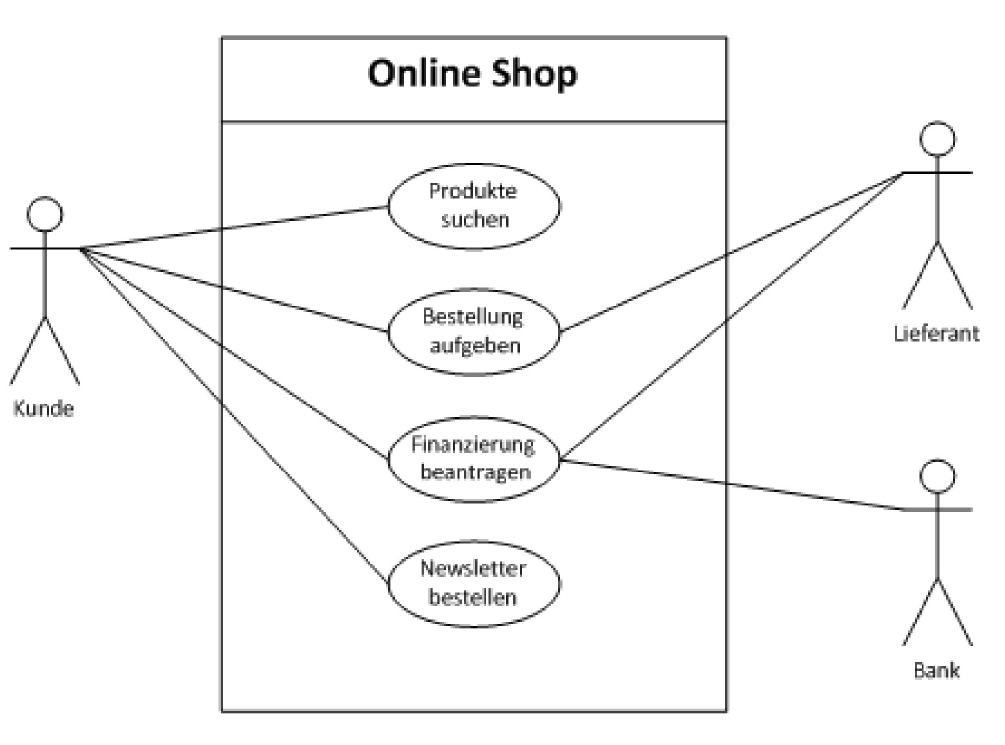
\includegraphics[width=0.65\textwidth]{Bilder/usecase.png}
			\caption[Beispiel eines UML-Diagramms f�r einen Anwendungsfall]{Beispiel eines UML-Diagramms f�r einen Anwendungsfall (nach \textcolor{red}{[11]})}
			%Quelle: http://andreas-pfund.de/konzeption/konzeption_methode_webseite/webseite_anwendungsfall_use_case.php
			\label{fig:usecase}
		\end{figure}
		
		% TODO
		%https://www.microtool.de/was-sind-use-cases/
		\vspace*{-0.5cm}
		
		\subsubsection*{Konzept \textit{Use Case 2.0}}
		
		Insbesondere im Kontext agiler Projektentwicklungs-Konzepte ist die Anzahl der potentiellen Use Cases jedoch h�ufig zu umfangreich, um innerhalb klassischer Projekt-Teilintervalle von wenigen Wochen (im Scrum-Kontext als \textit{Sprints} bezeichnet) aus den Projektbeschreibungen extrahiert und final implementiert zu werden.
		Zur L�sung dieser Problematik publizierten Ivar Jacobson, Ian Spence und Kurt Bittner im Dezember 2011 das Konzept der \textit{Use Cases 2.0} \textcolor{red}{[11]}. %Quelle: https://www.microtool.de/wie-funktioniert-use-case-2-0/
		Der monolithische Ansatz zur exhaustiven Use-Case-Generierung wird hierbei durch eine skalierbare, agile Technik zur sukzessiven Konkretisierung von Anforderungen substituiert, welche adaptiv an die Verfahrensparameter der inkrementellen System- und Produktentwicklung angepasst werden kann. Die konzeptionelle Grundlage zur agile Projektplanung mit Use Cases liefert dabei das \textit{Slicing}, welches die Zerlegung eines Use Cases in kleinere Teileinheiten beschreibt; die hierbei extrahierten Use-Case-Fragmente werden dabei so angepasst, dass ihre wesentlichen Bestandteile innerhalb eines Projektintervalls realisiert werden k�nnen \textcolor{red}{[11]}.\\ 
		%Quelle: http://www.erp-selection.ch/agiles-projektmanagement/				
		Die Segmentierung eines Use Cases wird dabei durch iterative Isolation koh�renter Interaktionsfolgen zwischen Aktor und Systeminstanz realisiert, welche final in der Extraktion autarker, stark konkretisierter Anwendungsf�lle resultiert. Diese repr�sentieren dabei h�ufig verschiedene, interne Ablauffolgen des analysierten Use Cases; der Grundgedanke der selektiven Pfadauswahl zur \textit{Slicing}-Realisierung ist in Abbildung \ref{fig:usecase2} unten dargestellt.\\
		
		\begin{figure}[h] 
			\centering
			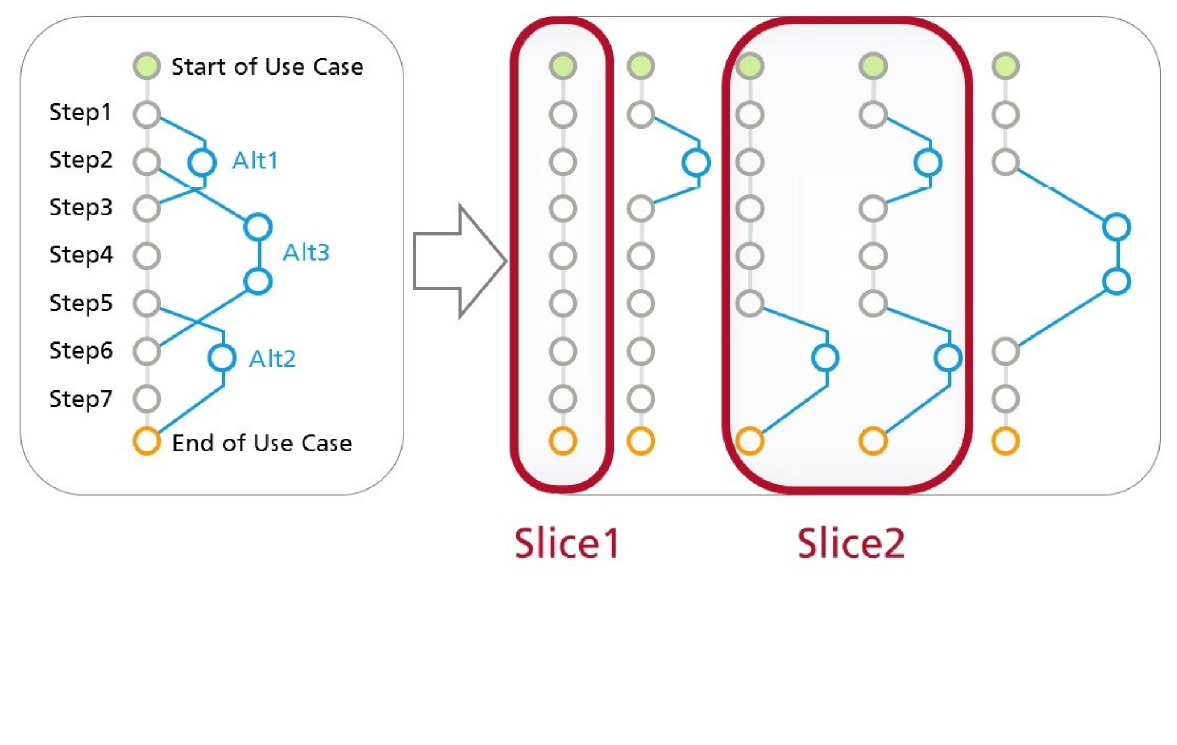
\includegraphics[width=0.85\textwidth]{Bilder/slices.png}
			\caption[Exemplarisches \textit{Slicing} eines monolithischen Use Cases]{Exemplarisches \textit{Slicing} eines monolithischen Use Cases \textcolor{red}{[11]}}
			%Quelle: http://andreas-pfund.de/konzeption/konzeption_methode_webseite/webseite_anwendungsfall_use_case.php
			\label{fig:usecase2}
		\end{figure}
		
		\noindent Zus�tzlich wird der Realisierungsaufwand individueller Teilaspekte der Anforderungen h�ufig unter Verwendung eines internen Punktesystems quantifiziert, um auf Basis einer initialen Aufwandsabsch�tzung die selektive Priorisierung ausgew�hlter Projektanteile zu erm�glichen. Auf diese Weise kann insbesondere die im agilen Projektkontext elementare Kommunikation mit den Auftraggebern verbessert werden, da Produktartefakte mit \mbox{wesentlichen} Funktionselementen zeitnah generiert und in ihrer Korrektheit (beispielsweise durch manuelle Kontrollen des jeweiligen Auftraggebers) verifiziert werden k�nnen \textcolor{red}{[11]}. % Quelle:  http://www.erp-selection.ch/agiles-projektmanagement/	
		
		
	\subsection{Perspektive: Kunde}
		
		In diesem Abschnitt werden die use-cases behandelt, welche aus Kundensicht aufkommen. Anhand eines Beispielszenarios, in dem ein Kunde Getr�nke bestellt und bezahlt, werden die einzelnen use-cases benannt und detailliert erl�utert. Auch Sonderf�lle, wie etwa die Stornierung eines Getr�nkes werden beachtet.\\
		Der durchschnittliche Kunde wird, nachdem er die Bar betreten hat, an einem Tisch platznehmen und dort die Cocktailkarte anschauen. Typischerweise sollten hier die Preise direkt neben den Cocktails stehen. Die Bestellkarte selbst ist online verf�gbar, auf der Website der Bar. Durch Ber�hren des gew�nschten Cocktails wird dieser zu einer Bestellliste hinzugef�gt. Diese Prozedur wiederholt der Kunde so lange, bis die gew�nschte Menge sowie Art an Cocktails auf der Bestellliste steht. Der Gesamtpreis sollte deutlich erkennbar angezeigt werden. Ein Button mit dem Text Bestellen signalisiert das Ende der Bestellung und initiert den tats�chlichen Einkauf. Das Format der Website muss an Mobiltelefone angepasst sein, da Kunden in der Regel mit diesen bestellen werden. Wird die Bestellung get�tigt, so werden die ben�tigten Daten an die Bar �bermittelt, sodass ein Mitarbeiter die entsprechenenden Cocktails zubereiten kann. Der Kunde bekommt eine visuelle Best�tigung auf der Website, dass seine Bestellung eingegangen ist und bearbeitet wird. Auch eine Zahlungsbest�tigung muss angezeigt werden. Die Bestellung selbst kann ebenfalls erneut aufgerufen werden, um f�r sp�tere �nderungen verf�gbar zu sein. Die Zahlung selbst verl�uft per Blockchain im Hintergrund und ist voll automatisiert. Hat der Kunde nicht genug Geld in seinem Wallet, so wird die Bestellung abgebrochen und ein entsprechender Hinweis wird angezeigt. M�chte ein Kunde, nachdem er eine Bestellung aufgegeben hat, die Anzahl oder Art der Cocktails �ndern, so muss er die gespeicherte Bestellung auf der Website aufrufen und durch entsprechende Interaktion die Anzahl oder Art der Cocktails ver�ndern. Die Differenz des Betrags wird daraufhin entweder an die Bar �berwiesen oder an den Kunden zur�ckerstattet. Eine entsprechende Best�tigung wird dem Barpersonal sowie dem Kunden angezeigt. Eine �nderung soll nur einmalig m�glich sein und, sofern die Bestellung ver�ndert wurde, als Notiz an die Bestellung angeheftet werden. Werden die Cocktails an den Kundentisch geliefert, so wird die Bestellung als abgeschlossen markiert und ist nicht mehr ver�nderbar. Ist ein Kunde mit der Bestellung unzufrieden, etwa wenn ein Cocktail nicht angenommen und daher auch nicht konsumiert wird, so muss es eine M�glichkeit der R�ckerstattung geben. Dies geschieht durch einen speziellen Button, welcher den Wunsch der R�ckersattung an die Website der Bar sendet. Dieser wird, nach Pr�fung durch das Personal, entweder gew�hrt oder gel�scht. Nach Konsum der Cocktails soll es dem Kunden m�glich sein, Trinkgeld an den Kellner zu �bermitteln. Dies wird, wie bereits mit zahlreichen Optionen davor, mit einem entsprechenden Button auf der Website signalisiert und ist nicht an eine bestimmte Bestellung gekoppelt. Ebenfalls wie bei einem normalen Einkauf geschieht diese �berweisung vollautomatisch und ist nicht reversibel. Eine Best�tigung der Trinkgeld�berweisung wird, nachdem die Transaktion erfolgreich abgeschlossen wurde, unterhalb des Trinkgeldbuttons angezeigt.	
			
	
	\subsection{Perspektive: Betreiber}
	

In diesem Abschnitt werden die UseCases behandelt, die aus Betreibersicht durch das Tool aufkommen. Zus�tzlich werden die Unterschiede zu herk�mmlichen Betrieben aufgezeigt, wie sie vielfach auftreten.\\
Sobald sich der Kunde an einen Tisch gesetzt hat, betrachtet er die Speisekarte, welche manchmal erst vom Wirt oder Kellner gebracht wird. Sobald sich der Kunde f�r ein Getr�nk oder eine Speise entschieden hat, tritt der Betreiber erneut an den Tisch und nimmt die Bestellung auf. Erst danach kann der Betreiber mit dem Zubereiten der Speisen oder dem Mixen der Getr�nke beginnen. Dies ist ein zeitaufw�ndiger Prozess. Mithilfe der Anwendung lassen sich Bestellung aus Betreibersicht automatisch verarbeiten. W�hrend der Kunde seine Tischnummer angibt und die Bestellung abgibt, werden die Informationen direkt an den Betreiber gesendet. Der Wirt sieht dann, welche Getr�nke zu welchem Tisch geliefert werden m�ssen. Dies vermindert die Zeit der Bestellungsaufnahme erheblich und der Wirt hat mehr Zeit, sich um seine Kernkompetenzen zu k�mmern, dem Mixen von Getr�nken. Zus�tzlich kann der Kunde auch angeben, dass er die Beratung eines Wirtes sucht oder einen Spezialwunsch hat, sodass der Betreiber auf individuelle W�nsche des Kunden eingehen kann und den Kontakt aufrecht erh�lt. Damit bleibt der Prozess, trotz der Strukturierten Blockchain mit starren Produkten und Preisen, ein sehr dynamischer Vorgang, der bei Bedarf angepasst werden kann. \\
Die Buchhaltung ist in Gastronomiebetrieben sehr komplex, da verschiedenste Rechnungen miteinander verbunden werden m�ssen. In kleineren Betrieben wird die Abrechnung gr��tenteils auf Papier erstellt. In mittelgro�en bis gro�en Betrieben, dient eine Software zur Bearbeitung von Rechnungen. Mithilfe der Blockchain Technologie erfolgt die Abrechnung binnen k�rzester Zeit. Direkt nach der Bestellung, wird der Kunde gebeten den zu entrichtenden Betrag zu zahlen. W�hrend dem Kunden nur der endg�ltige Betrag gezeigt wird, wird intern eine aufgeschl�sselte Rechnung gespeichert. So k�nnen genau Materialkosten, Personal, Steuern und sonstige in der Rechnung enthaltenden Betr�ge angezeigt werden. Dies erleichtert die Abrechnung erheblich. Durch die in der Blockchain gespeicherten Informationen k�nnen die Rechnungen auch nach langer Zeit noch nachvollzogen und begr�ndet werden. Auch ist es m�glich, Trinkgelder in den Betr�gen anzugeben und diese bei der Abrechnung zu ber�cksichtigen. Diese L�sung bietet auch kleineren Betrieben die M�glichkeit, ihre Abrechnung digital und einfach zu speichern und dann weiterzuverarbeiten.\\
Die Webanwendung erm�glicht au�erdem die Anpassung der Speisekarte. Normalerweise m�ssen alle Speisekarten bei ge�nderten Preisen neu ausgedruckt werden. Bei Sonderangeboten wird beispielsweise ein zus�tzliches Blatt in die Speisekarte gelegt oder eine eigene Tageskarte erstellt. Dieser Prozess ist sehr kostspielig und auch zeitintensiv. Fehler in der Speisekarte k�nnen nur mit viel Aufwand wieder korrigiert werden. \\
Um beispielsweise neue Produkte der Speisekarte hinzuzuf�gen oder Preise anzupassen ist eine Ver�nderbarkeit der Speisekarte in der Webanwendung erforderlich. Dadurch ist es m�glich, verschiedene Sonderangebote oder neue Produkte ohne Zeitverz�gerung in das System einzupflegen und den Kunden direkt die neue Speisekarte zur Verf�gung zu stellen. Die Kunden m�ssen dabei keine neue Seite Aufrufen, da sich die Webseite automatisch aktualisiert und die ge�nderten Preise und Produkte in Echtzeit anzeigt. Die Anwendung l�sst sich auch mit herk�mmlichen Speisekarten kombinieren, sodass ein autarker Betrieb m�glich ist. \\
Durch den gro�en Bekanntheitsgrad der Blockchain in den vergangenen Jahren dient das Benutzen dieser Technologie im eigenen Betrieb als gutes Werbemittel \cite{faizod1}. Viele Nutzer sehnen sich au�erdem nach Anwendungen f�r die Blockchain \cite{wiwo1}. Sollte eine Gastronomieunternehmen nun bekannt geben, dass es auch eine M�glichkeit zu Bestellung und Bezahlung �ber die Blockchain erm�glichen, so wird es durch das Alleinstellungsmerkmal neue Kunden gewinnen. Manche Kunden werden allein aufgrund der Technologie und nicht den eigentlichen Produkte das Gesch�ft betreten und die Anwendung testen. Dies wiederum erm�glicht ein Feedback von Nutzern, die sich gut in dem Bereich Blockchain auskennen, was die Anwendung verbessert und Fehler behebt.\\


\noindent Alle diese UseCases lassen sich problemlos auch mit dem herk�mmlichen Betrieb der Gastronomie verbinden. So sind Kunden nicht auf die Blockchain-Technologie angewiesen. Dies erleichtert Personen, die sich nicht mit dem Thema besch�ftigen wollen, einen normalen Besuch, ohne mit der Blockchain in Ber�hrung zu kommen.
	
	\chapter{\label{chap:5proto}Implementierungsprotokoll Demonstrator-App}
	
	\section{Aufbau}
	
		F�r den Prototyp eignet sich besonders die Ethereum-Blockchain, da diese die Verwendung von Smart-Contracts auf der Ethereum-Virtual-Machiene (EVM) zul�sst und gleichzeitig �ber eine eigene W�hrung verf�gt. So kann das Senden von Transaktionen mit einer Logik verkn�pft und automatisiert werden. 
		Die Berechnungen der Smart-Contracts werden innerhalb einer Virtuellen-Maschine bei den Minern ausgef�hrt. Als Ausgleich bezahlt der Absender einer Transaktion einen kleinen Betrag. 
		Es kann angenommen werden, dass beim Bezahlen einer Geb�hr von ca. 15 Cent (Stand Januar 2018) die Transaktion innerhalb einer Minute von der Ethereum-Blockchain verarbeitet wird. Diese Geb�hr ist Abh�nig von der Anzahl der Speicher- und Rechenoperationen. Deshalb sollte der Zustand einer Variable auf der Blockchain nur dann ver�ndert werden, wenn dies auch wirklich n�tig ist. 
		
		Im folgenden Kapitel wird die Implementierung einer DApp beschrieben, also einer Decentralized Application. Decentraliczed Applications bieten eine Schnittstelle zwischen Blockchain und Anwender. Nicht immer ist die Interaktion mit Smart-Contracts f�r den Nutzer durch ein Wallet intentional oder �bersichtlich. Es ist m�glich, dass Datentypen falsch verwendet werden und der Nutzer im schlimmsten Fall finanziellen Schaden nimmt. Deshalb bieten DApps eine grafische Benutzeroberfl�che, die Beispielsweise auf einem Webserver zur Verf�gung gestellt wird. So k�nnen auch unerfahrene Nutzer ohne technisches Vorwissen mit der DApp interagieren. Durch Wallets wie MetaMask kann eine Verbindung zwischen dem Ethereum-Account und der DApp hergestellt werden. 
		
		Zur Entwicklung des Smart-Contracts wird bei der Entwicklung des Prototypen die Programmiersprache Solidity verwendet. Die Syntax ist von der Javascript-Notation abgeleitet. Beim Kompilieren eines oder mehrerer Solidity-Files entsteht Bytecode, welcher auf der EVM ausgef�hrt werden kann. 
		Die Schnittstelle zwischen Ethereum und Javascript wird durch die Web3-Bibliothek gew�hrleistet. Diese wird verwendet, um die Verbindung zwischen Frontend und den auf der Blockchain gespeicherten Daten herzustellen. 
		
	\section{Smart-Contracts}	
	
		Das folgende Kapitel besch�ftigt sich mit der Entwicklung des Smart-Contracts. 
		Dieses Kapitel stellt die Grundlage der Implementierung dar. Mit der verwendeten Programmiersprache Soldity  k�nnen sogenannte Contracts, also Vertr�ge, definiert werden. Diese werden entweder einzeln oder kaskadiert auf der Blockchain ausgef�hrt. Deshalb wird Solidity auch als Vertrags-Orientiert betitelt \cite{soliditydoc}.
		
		Die Ausf�hrung des Programmcodes wird durch die Einheit Gas verg�tet \cite{Wood-2017}. Das verbrauchte Gas pro Rechen- oder Speicheroperation wird mit dem angegebenen GasPreis multipliziert und muss mit dem Befehl zum Ausf�hren des Smart-Contracts an die Miner entrichtet werden. 
		Smart-Contracts werden einmal initial an die Blockchains gesandt und der Konstruktor wird ausgef�hrt \cite{EthWP-2017}.
		
		Sobald der Smart-Contract auf der Blockchain ist, k�nnen andere Teilnehmer �ber die sogenannte Application Binary Interface (ABI) auf den Smart-Contract zugreifen und dessen Funktionen ausf�hren. 
		
		Der Smart-Contract selbst ist auf die EVM  limitiert. Zwar gibt es globale Einheiten, wie die Zeit in Sekunden, welche seit dem ersten Block vergangen ist messen, jedoch besitzt die EVM kein Zugriff auf externe Speichermedien \cite{soliditydoc}. Zur Abbildung monet�rer Vorg�nge ist mit Solidity die Umrechnung in die Untereinheiten von Ethereum wie zum Beispiel in Wei m�glich. 
		Dies ist notwendig, wenn wir beispielsweise einen Betrag an den Smart-Contract schicken m�chten. Jeder Smart-Contract hat einen eigenen Public-Key und kann �ber Funktionen, die mit dem Schl�sselbegriff \texttt{payable} markiert wurden, die Bezahlung in ETH empfangen. Dieser Betrag wird grunds�tzlich in Wei gesendet. Eine Umrechnung ist in der Tabelle \ref{table:values} zu sehen. Diese Aufteilung ist notwendig, um Nachkommastellen von Ethereum Betr�gen entsprechend darstellen zu k�nnen, da in der aktuellen Version Flie�kommazahlen nicht unterst�tzt werden \cite{floating}.
		
		\begin{center}
			\captionof{table}{Untereinheiten der Ethereum-W�hrung}
			\begin{tabular}{ | c | c | }
				\hline
				Multiplizierer & Name\\ \hline
				\(10^0\) & Wei \\ 
				\(10^{12}\) & Szabo \\ 
				\(10^{15}\) & Finney \\ 
				\(10^{18}\) & Ether \\
				\hline
			\end{tabular}
			\label{table:values}
		\end{center}
		
		Der Smart-Contract der DApp soll m�glichst die Bestellung aufnehmen k�nnen, den entsprechenden Betrag errechnen und den Nutzer dann die M�glichkeit geben, den Betrag zu bezahlen. Der Contract muss jedoch in seiner Funktionalit�t schlicht gehalten werden, da, wie bereits erw�hnt, Rechenleistung sehr teuer werden kann. Es muss also versucht werden, die �bertragungskosten im Verh�ltnis zu den Kosten des Services m�glichst klein zu halten. 
		
		Zus�tzlich sollte beachtet werden, dass der Besitzer des Smart-Contracts besondere Privilegien erh�lt. In der Regel wird der Initiator des Smart-Contracts jedoch nicht zwangsl�ufig der Besitzer des Restaurants sein oder der Besitzer des Restaurants wechselt, weshalb eine Funktion zum �bertragen  der Privilegien n�tig ist. Diese Funktionalit�t wird in der \texttt{transferPriv}-Funktion gew�hrleistet (siehe Listing \ref{lst:def}).
		Diese Privilegien k�nnen es beispielsweise erm�glichen, die Aussch�ttung des Gewinnes auszul�sen oder den Preis einzelner Produkte zu �ndern und neue hinzuzuf�gen. 
		
		\begin{lstlisting}[caption={Drinks: defining manager},label=lst:def]
		pragma solidity ^0.4.17;
		
		/**
		* @title Drinks, the one and only Bar-DApp
		* @dev Version of the Drinks-Contract for the "IT-Management" project
		*/
        contract Drinks {
		
		address public manager;
		mapping(uint => mapping (uint => uint)) public orders;
		mapping(uint => uint) public prices;
		
		event EmptyPay(address _sener, uint _amount);
		
		/**
		* @dev Set msg.sender as manager
		* @dev Set prices for drinks in ether
		*/
		function Drinks() public {
		manager = msg.sender;
		prices[0] = 0.7 ether;
		prices[1] = 0.5 ether;
		prices[2] = 0.3 ether;
		prices[3] = 0.1 ether;
		}
		
		/**
		* @dev Select a new manager 
		* @param _manager new manager
		*/
		function transferPriv(address _manager) public payable {
		manager = _manager;
		}
		\end{lstlisting}
		
		Nachdem der Besitzer festgelegt ist, werden in der Funktion \texttt{Drinks} die Preise f�r die Produkte festgelegt. Um diese nachtr�glich zu ver�ndern oder zu erg�nzen, kann die Funktion \texttt{changePrice} aufgerufen werden (siehe Listing \ref{lst:price}). Die Anforderung f�r das �ndern der Preise ist, dass der Absender der Nachricht (\texttt{msg.sender}) auch der Manager des Vertrags ist. 
		
		Die \texttt{calcPrice}-Funktion zur Berechnung des Preises wird unabh�ngig von der Bezahlfunktion gehandhabt, da sie so auch im voraus vom Nutzer aufgerufen werden kann, um dem Nutzer den zu bezahlenden Betrag anzuzeigen (siehe Listing \ref{lst:price}). Der Nutzer �bergibt die ID und die Anzahl der Produkte als Array an die Funktion. Dies ist f�r wenige Produkte zwar speicheraufwendig, da gegebenenfalls bei einer Bestellung von nur einem Produkt bereits ein Array erzeugt werden muss. Es l�sst jedoch zu, dass der Besitzer weitere Produkte zur Getr�nkekarte hinzuf�gen kann, ohne den Smart-Contract in seiner Funktionalit�t zu beeinflussen. 
		In der Funktion selbst werden alle Preise mit der entsprechenden Anzahl an Items verrechnet und die Summe als \texttt{unsigend Integer} zur�ckgegeben. Die Funktion wird mit einem sogenannten \texttt{view}-Modifizierer versehen. Das bedeutet, dass die Funktion garantiert, keine Ver�nderungen an der Blockchain durchzuf�hren. So entstehen dem Nutzer beim Ausf�hren der Funktion keine Kosten. Die Ausf�hrung der Funktion muss daher auch nicht explizit durch den Nutzer genehmigt werden. 
		
		
		\begin{lstlisting}[caption={Drinks: price-functions},label=lst:price]
		/**
		* @dev Set a new Price
		* @param _drinks id of the drink
		* @param _amounts new price of the drink
		*/
		function changePrice(uint _drink, uint _price) public view returns (uint) {
		require(msg.sender == manager);
		prices[_drink] = _price;
		}
		
		
		/**
		* @dev Calculates the correct price of Drinks ordered
		* @notice Please call the calcPrice-Function first, and send the right Amount of Ether
		* @notice Contract will be reverted otherwise
		* @param _drinks provide array of listed drinks
		* @param _amounts array of ordered amounts
		* @return uint, price of coctails in Ether 
		*/
		function calcPrice(uint[] _drinks, uint[] _amounts) public view returns (uint) {
		uint price;
		for (uint i = 0; i < _drinks.length; i++){
		price += _amounts[i]* prices[_drinks[i]];
		}
		return price;
		}
		\end{lstlisting}
		
		Der Kern des Vertrages bietet die Bezahlfunktion \texttt{takeOrder} f�r die Produkte (siehe Listing \ref{lst:ordering}). Als Parameter der Funktion muss angegeben werden, f�r welchen Tisch die Bestellung aufgegeben wurde. Die Herausforderung liegt an dieser Stelle, wie bereits bei der Berechnungsfunktion, in der Darstellung und in der Speicherung der bestellten Getr�nke. Je nach Anzahl der insgesamt verf�gbaren Produkte auf der Karte empfiehlt es sich, entweder eine Aufreihung der Anzahl aller Getr�nke anzugeben, dabei jede ID als einfachen \texttt{Integer}-Wert. Jedoch w�rden dann auch ein \texttt{Integer} �bergeben werden, falls kein Produkt bestellt wurde. Mit wachsender Anzahl an Produkten auf der Getr�nkekarte lohnt sich daher ein Mapping. Dies l�sst auch ein einfaches Erweitern der Speisekarte zu, kostet aber bei der Ausf�hrung eine minimal h�here Summe an Gas. Da es sich jedoch im Anwendungsfall lediglich um einstellige Centbetr�ge handeln wird, wird dies als vernachl�ssigbar betrachtet. 
		Um die M�glichkeit zu gew�hrleisten, dass auch etwas f�r den Nachbartisch bestellt werden kann, wird die Tisch-ID, die im User-Interface ausgew�hlt wird, als Prim�rschl�ssel f�r die Speicherung der Getr�nke verwendet.
		
		Die Bezahlfunktion nutzt abschlie�end die Berechnungsfunktion, um zu �berpr�fen, ob der bezahlte Betrag in Wei dem zuvor berechneten Betrag entspricht. Sollte das nicht der Fall sein, wird die Funktion abgebrochen und das verbleibende Geld wird dem Nutzer zur�ckerstattet. 
		Danach wird durch alle Getr�nke durchitteriert und die entsprechende Menge auf der Blockchain hinterlegt. 
		
		Auch dem Personal muss die M�glichkeit gegeben werden, die Anzahl der bestellten Getr�nke abzurufen. Daf�r steht die \texttt{getOrder}-Funktion bereit (siehe Listing \ref{lst:ordering}). Dabei handelt es sich erneut um eine reine \texttt{view}-Funktion, da zu ihrer Ausf�hrung die Blockchain nicht ver�ndert werden muss. Mit ihr kann jeweils nur ein Getr�nk abgerufen werden, da die R�ckgabe von dynamischen Arrays und Mappings nicht unters�tzt wird \cite{soliditydocs}. Da die Ausf�hrung der Funktion jedoch kostenlos ist, kann diese Funktion iterativ f�r jedes Produkt aufgerufen werden. 
		
		Ist der Kunde bedient, kann die Bestellung �ber die \texttt{serve}-Funktion wieder von der Blockchain gel�scht werden (siehe Listing \ref{lst:ordering}). Auch hier werden wieder zwei Arrays und die ID des Tisches �bergeben. Die Anzahl wird hier nicht zur�ck gesetzt sondern lediglich um angegebene Anzahl verringert, sodass die Bestellung in mehreren Teilen erfolgen kann. 
		
		Zuletzt steht die Fallback-Funktion, die aufgerufen wird, wenn versehentlich Geld an den Smart-Contract geschickt wird, ohne eine Funktion aufzurufen. Das Geld kann dann zur�ckgesendet werden. 
		
		\begin{lstlisting}[caption={Drinks: order, server and fallback-functions},label=lst:ordering]
		/**
		* @dev Token-transfer from msg.sender to address
		* @notice Please call the calcPrice-Function first, and send the right Amount of Ether
		* @notice Contract will be reverted otherwise
		* @param _drinks provide array of listed drinks
		* @param _amounts array of ordered amounts
		*/
		function takeOrder(uint _table, uint[] _drinks, uint[] _amounts) public payable {
		uint price = calcPrice(_drinks, _amounts);
		require (msg.value >= price);
		for (uint i = 0; i < _drinks.length; i++){
		orders[_table][_drinks[i]] += _amounts[i];
		}
		}
		
		/**
		* @dev Returns the correct amount of coctails ordered from specific address
		* @param _table id of table
		* @param _drinkId id of requested drink
		* @return uint, amount of drinks
		*/
		function getOrder(uint _table, uint _drinkId) public view returns (uint){
		return orders[_table][_drinkId];
		}
		
		/**
		* @dev Removes ordered cotails from list
		* @notice Please do not call this contract if you arent the restaurant manager
		* @param _drinks provide array of served drinks
		* @param _amounts array of served amounts
		*/
		function serve(uint _table, uint[] _drinks, uint[] _amounts) public {
		require(msg.sender == manager);
		for (uint i = 0; i < _drinks.length; i++){
		orders[_table][_drinks[i]] -= _amounts[i];
		}
		}
		
		/**
		* @notice Fallback. Do not call this function ever. Thanks. 
		*/
		function() public payable { EmptyPay(msg.sender, msg.value); }
		
		} 
		\end{lstlisting}
		
	\subsection{Entscheidungen f�r das User Interface}	
	
		Dem Design des Frontendes wird hierbei eine besondere Rolle zugeteilt. Er muss die Einfachheit des Smart-Contracts durch eine simple aber funktionierende Nutzerschnittstelle erg�nzen. Die Blockchain-Technik wird noch lange nicht von jedem Nutzer akzeptiert, deshalb soll die Hemmschwelle besonders niedrig gehalten werden. 
		
		Um dies zu erm�glichen, ist die Entscheidung gefallen, zwei Front-End-Anbindungen zu erstellen. Zum einen f�r den Besucher des Restaurants, welches in Abbildung \ref{abb:visitor} dargestellt ist.  Zum anderen die Ansicht f�r die Mitarbeiter des Restaurants. Diese ist in Abbildung \ref{abb:member} zu erkennen.
		
		
		\begin{figure}[h]
			\centerline{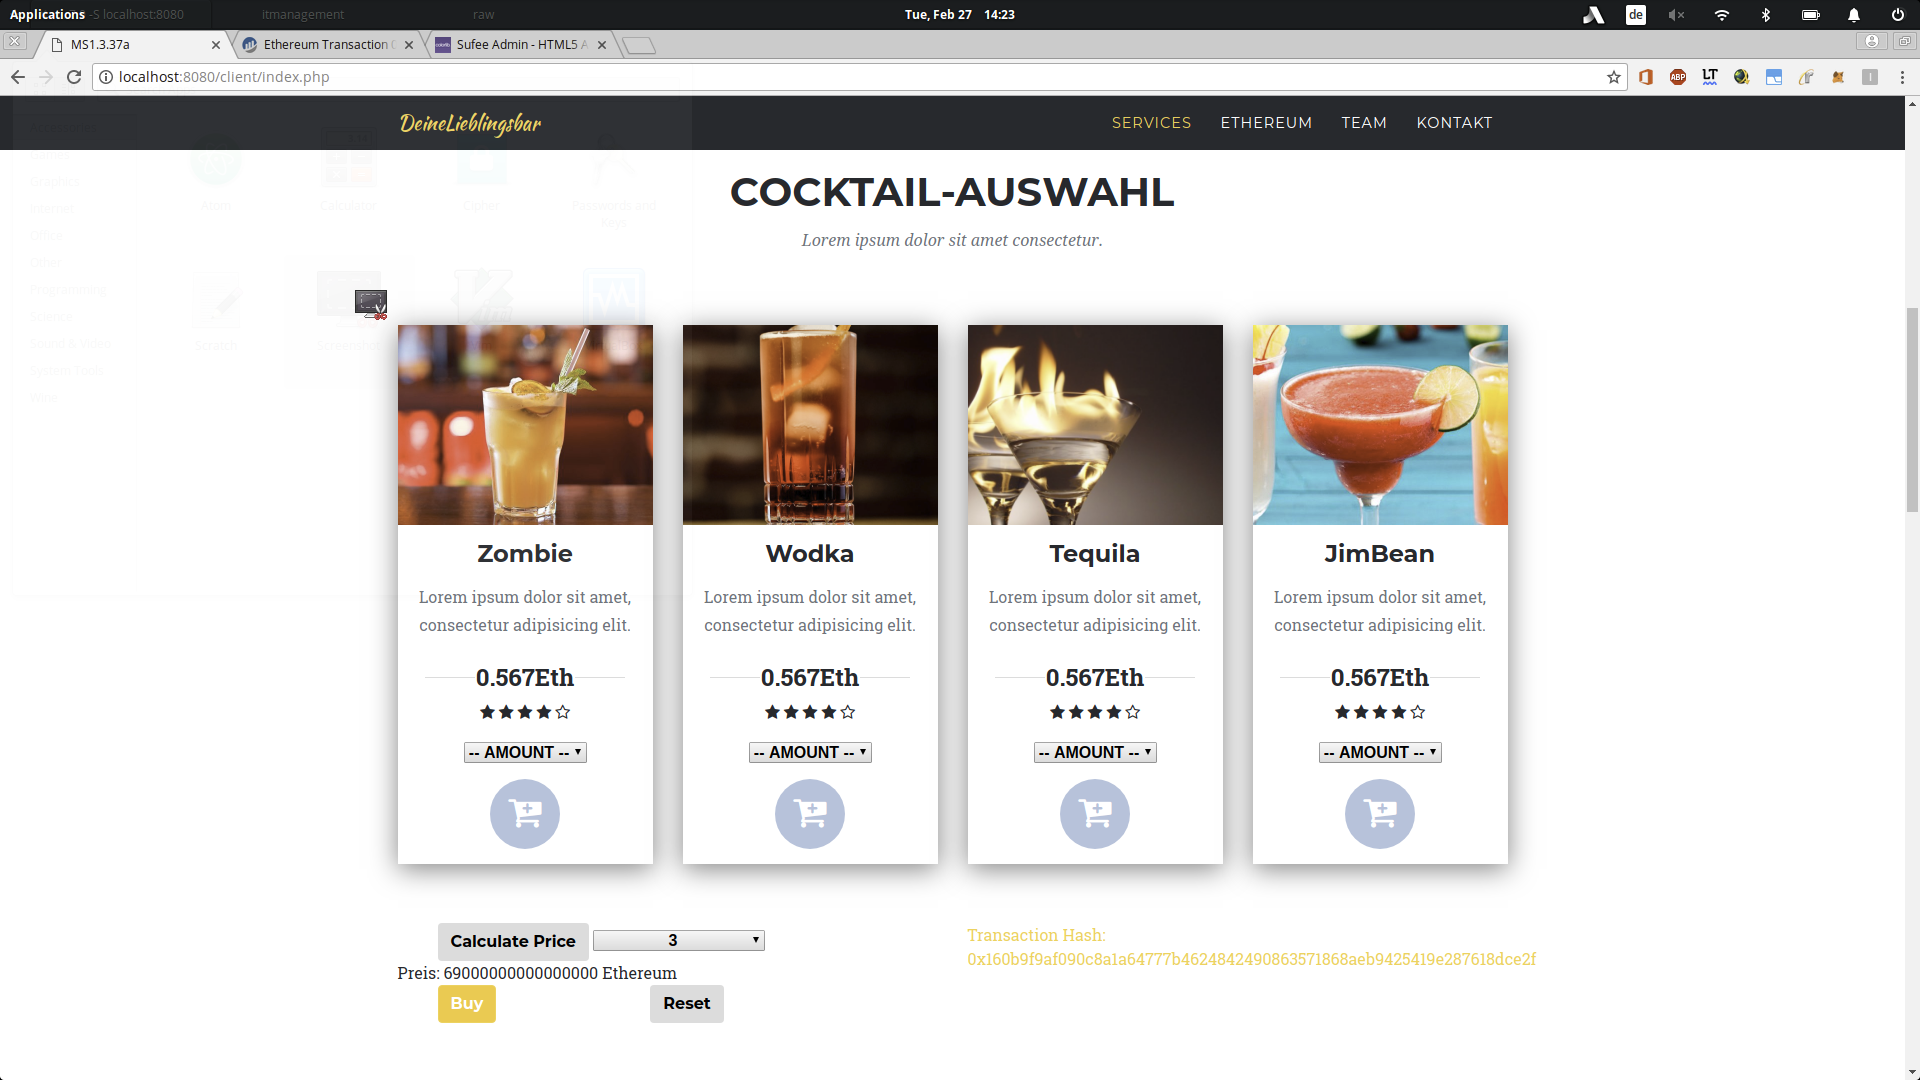
\includegraphics[width=15cm]{Bilder/screenshot1.png}}
			\caption{Ansicht f�r Besucher}
			\label{abb:visitor}
		\end{figure}
		
		\begin{figure}[h]
			\centerline{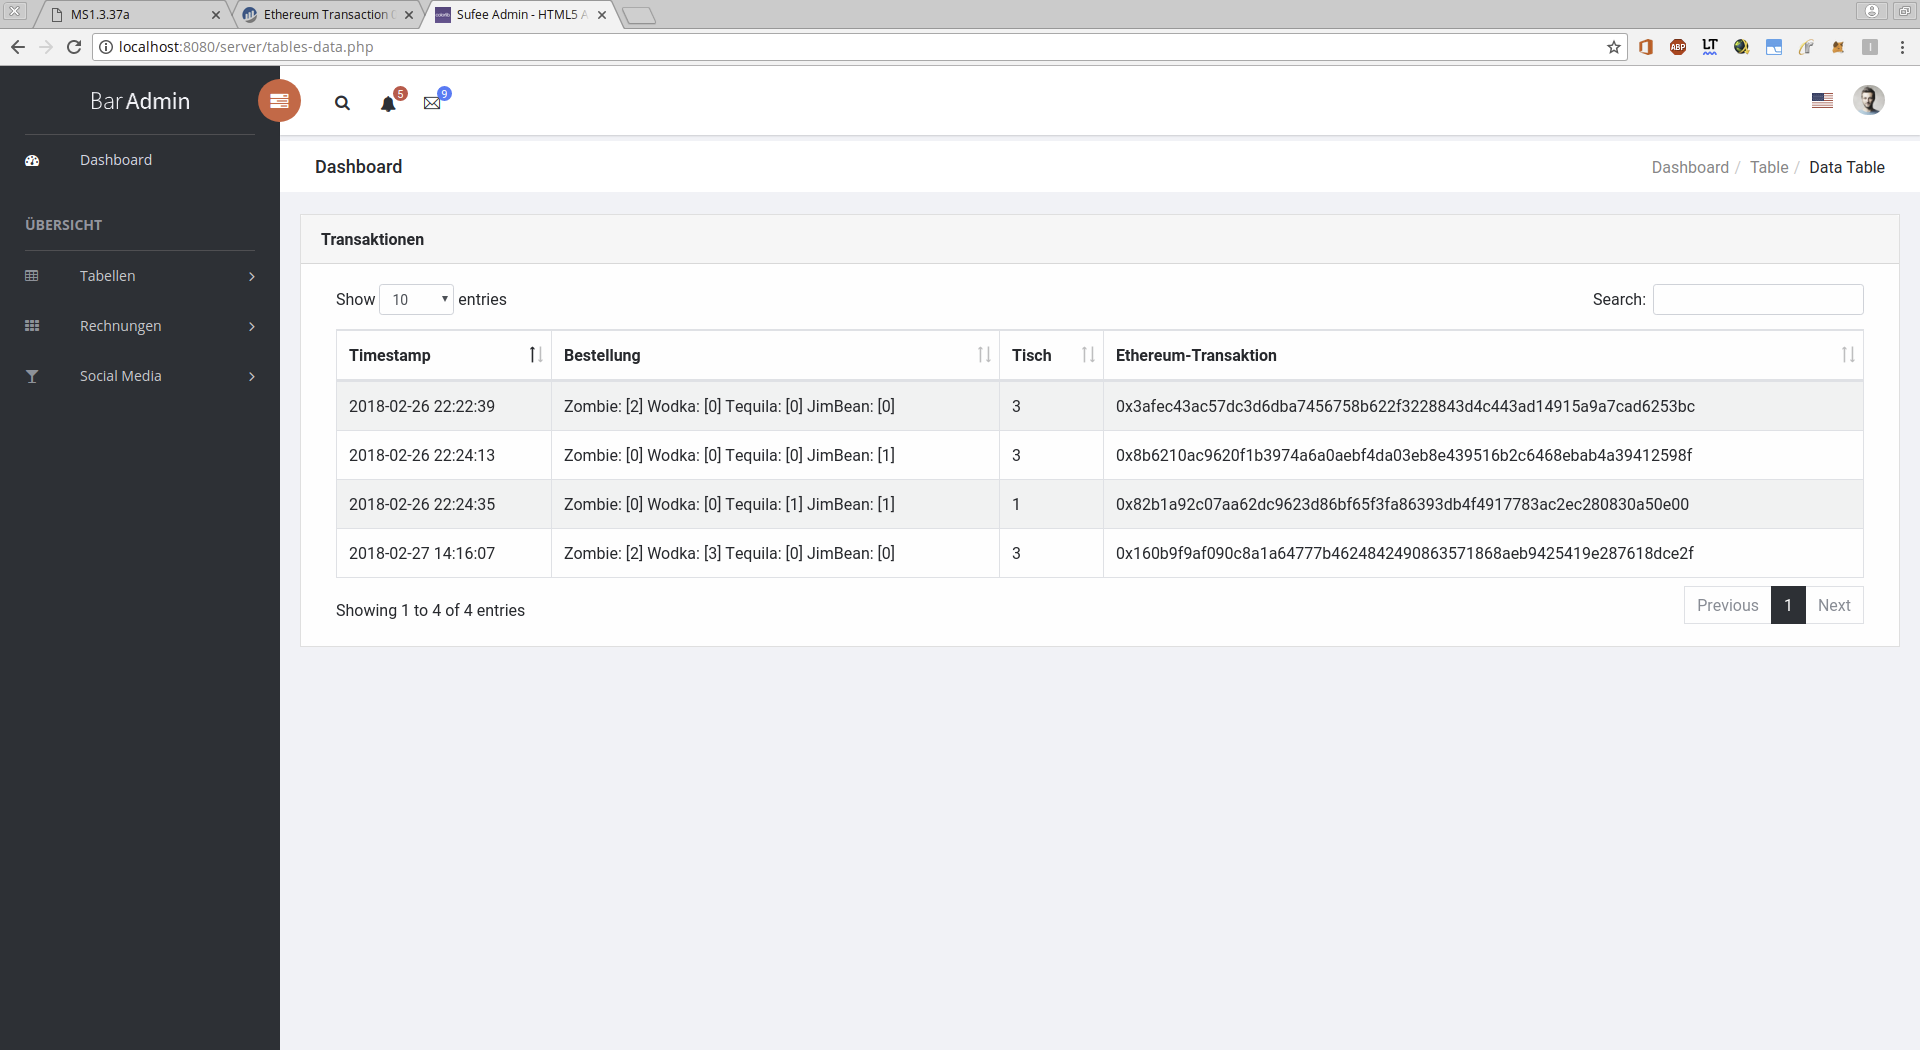
\includegraphics[width=15cm]{Bilder/screenshot3.png}}
			\caption{Ansicht f�r Mitarbeiter: Gesamt�bersicht}
			\label{abb:member}
		\end{figure}
		
		
		Die Frontend-Anbindung des Nutzers ist so gestaltet, dass sich der Nutzer die gew�nschten Produkte aus der Men�karte w�hlen kann und zu einem Warenkorb hinzuf�gen kann. Hat der Nutzer den Auswahlvorgang abgeschlossen, so kann er �ber den Men�-Button \glqq Preis berechnen \grqq{} die Blockchain-Funktionalit�t nutzen, um den exakten Preis zu berechnen. Dies wird �ber die Funktionalit�t der Blockchain gel�st, da so sichergestellt werden kann, dass exakt dieselben Parameter verwendet werden und die Transaktion nicht fehlschl�gt. Ist der Nutzer mit dem Preis einverstanden, kann er die Transaktion er�ffnen. 
		Dabei �ffnet sich die Metamask Integration, welche den erwarteten Preis bereits anzeigt. Der Nutzer braucht lediglich die Transaktion best�tigen. 
		Um dem Nutzer eine Best�tigung zu geben, wird der Transaktion-Hash angezeigt und auf Etherscan verlinkt \cite{etherscan}. Eine Ansicht dessen findet sich in Abbildung \ref{abb:etherscan}.
		Dort kann er nun �berpr�fen, ob die Transaktion schon angenommen wurde oder ob diese noch ausstehend ist. Ein Mitarbeiter k�nnte sich nun die Transaktion einscannen und die Bezahlung �berpr�fen. 
		
		\begin{figure}[h]
			\centerline{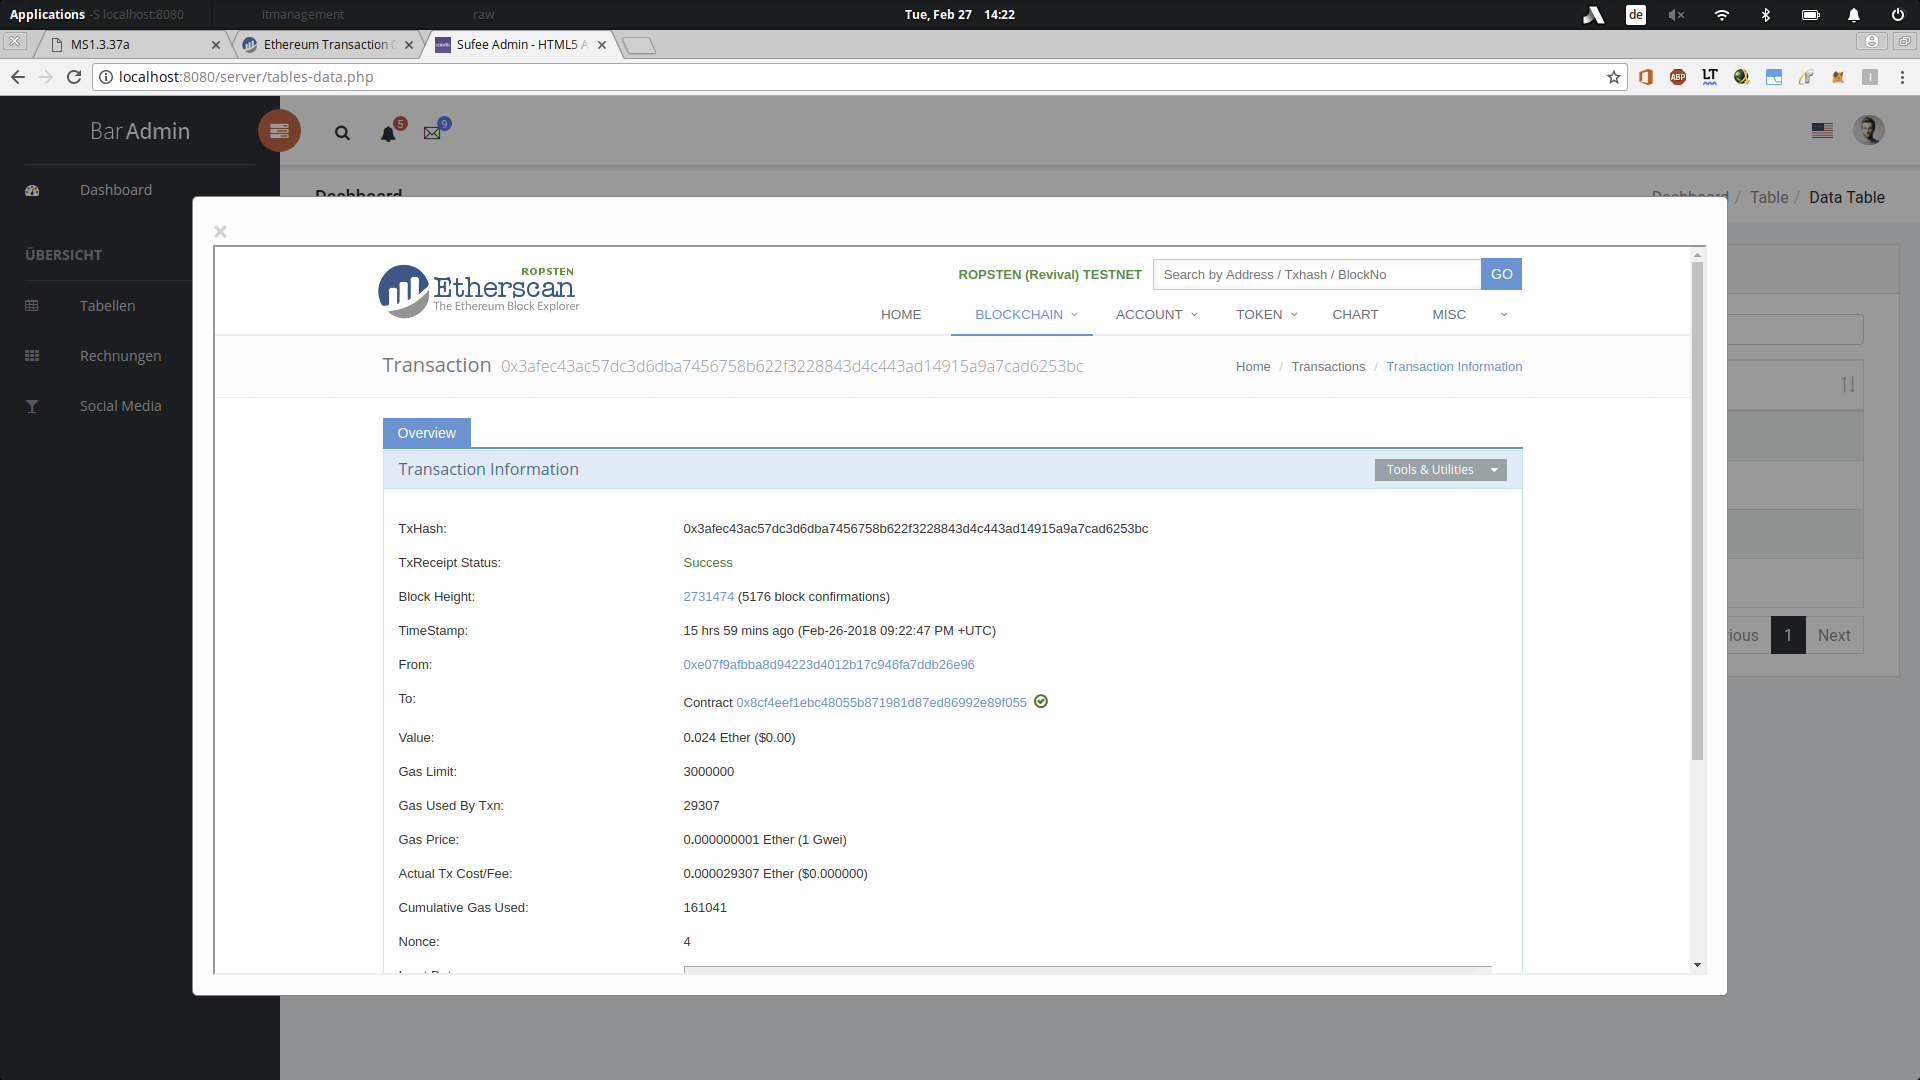
\includegraphics[width=15cm]{Bilder/screenshot2.png}}
			\caption{Ansicht f�r Mitarbeiter: Verifikation durch Etherscan}
			\label{abb:etherscan}
		\end{figure}
		
		Die Mitarbeiter, welche die Bestellung aufnehmen, und verarbeiten erhalten eine gesonderte Ansicht. Im Hintergrund werden die relevanten Daten der Bestellung, inklusive des Transaction-Hashs, in eine Datenbank eingetragen. Dies darf nur nach erfolgreicher Bezahlung erfolgen. Der Absender der Nachricht ist zwar in der Transaktion hinterlegt, jedoch ist diese Information f�r die Bestellung nicht weiter relevant, da der entsprechende Tisch angegeben wurde. Als Primary-Key dient der Datenbank eine fortlaufende Nummerierung der Transaktion-Hash. Dieser wird zus�tzlich als Link hinterlegt und kann bei bedarf �berpr�ft werden. Falls ein Fehler unterlaufen sollte, k�nnte das Personal den tats�chlichen Absender des Geldes ermitteln, vorausgesetzt der K�ufer gibt seine Ethereum-Addresse preis. Auch eine manuelle R�ckzahlung w�re dadurch m�glich. Desweiteren muss die Auflistung selbstverst�ndlich die bestellten Getr�nke enthalten.
	
	% Evaluation
	%\chapter{Evaluation}	

Um die Bewertungen des Szenarios und die daraus abgeleiteten Priorit�tensch�tzungen aus Technologie und Anwendbarkeit nachvollziehen zu k�nnen, wurden mit verschiedenen Gastronomien Experteninterviews durchgef�hrt, bei denen diese �ber das Thema Blockchain und dem Einsatz in der Gastronomie befragt und dar�ber hinaus qualitative Fragen zu den einzelnen Einflussfaktoren entsprechend der Anwendbarkeit und dem Nutzen
beantworteten. Die Experteninterviews dienen somit auch zur Plausibilit�tspr�fung des generierten Modells und der subjektiven Bewertungen der Befragten. Damit kann �berpr�ft werden, ob das Modell g�ltig, in der
vorliegenden Form annehmbar und nachvollziehbar ist \cite{Glaeser2010}. 

\section{Durchf�hrung der Interviews}

Die Frageformulierung und der Aufbau des Fragebogens erfolgen in Form
eines strukturierten Leitfrageninterviews. Dabei wurden die wichtigsten Themen als Fragen formuliert, aber bewusst Raum f�r tiefer gehende Fragen gelassen. Die nachfolgende Tabelle \ref{TabelleFragen} zeigt die vordefinierten Themen, die das Interview behandelt und auf welche n�her eingegangen werden kann. 

\begin{table}[h]
	\caption{Themen f�r die Experteninterviews}		
	\renewcommand{\arraystretch}{1.2}
	\begin{center} 
		\begin{tabular}{| p{5cm} | p{7cm} |}
			
			\hline
			\textbf{Blockchain}	& Grundlagen Blockchain \\
			& kryptografischer Hintergrund \\
			& Wissenstand Kryptow�hrung \\
			\hline
			
			\textbf{derzeitige Situation} 	& Durchf�hrung Bestellvorgang\\
			& Abwicklung Bezahlung \\
			& Abrechnung nach Bezahlung \\
			& Trinkgeld \\
			& Webauftritt \\
			\hline	
			
			\textbf{Szenario}	& Vorstellung des Szenario \\
			& �nderung am System \\
			& Vor-/Nachteile\\
			& Anwendbarkeit f�r Betrieb\\
			
			\hline
			
			
		\end{tabular}
	\end{center}
	\label{TabelleFragen}		
\end{table}

\noindent In besonderem Ma�e sind die Antworten zum Thema der Anwendbarkeit wichtig f�r die Auswertung, weshalb dort auf eine detaillierte Begr�ndung Wert gelegt wird.\\
Folgende Betriebe im Bereich Gastronomie wurden befragt:

\begin{itemize}
	\item Unicasino Unibw, Neubiberg
	\item Taverne Artemis, Ottobrunn
	\item Die 2, Neubiberg
	\item La Ciacolada, Neubiberg
	\item Santorini, Naumburg
	\item Landgasthof alter Bahnhof, Rohrberg
\end{itemize}

Alle Betriebe befinden sich in D�rfern oder Kleinst�dten. W�hrend \textit{Die 2} haupts�chlich als Bar dient und das \textit{Unicasino} eine separate Bar besitzt, sind die restliche 4 Gastronomien ausschlie�lich Gastst�tten beziehungsweise Restaurants. �ber Kundenzahl und Umsatz sind keine Informationen bekannt.\\
Nachdem alle Daten erhoben wurde, wurde eine Reduktion auf die wichtigsten Aussagen getroffen, welche weiter untersucht werden. Beim Thema Blockchain fiel sofort auf, dass es eine starke Diversifikation im Wissenstand der Befragten gab. W�hrend die Betreiber von \textit{Die 2} ein etwas umfangreicheres Wissen �ber Blockchain und Kryptow�hrungen besa�en, einer von ihnen besch�ftigt sich auch mit der Kryptow�hrung Ethereum, interessiert die Befragten des \textit{Unicasinos} und der Taverne \textit{Artemis} das Thema ein wenig und sie verstehen die Blockchain im groben. die restlichen 3 Betriebe haben nur durch Nachrichten die Begriffe schon einmal geh�rt. Alle sechs Betriebe assoziierten den Begriff der Blockchain fast ausschlie�lich nur mit Kryptow�hrungen und spekulativen Investments. Eine gro�e Gemeinsamkeit aller Betriebe ist die derzeitige Situation in Bezug auf Bestellung, Bezahlung und der Abwicklung von Rechnungen. Die Bestellung l�uft durch einen Kellner, der pers�nlich an den Tisch geht und die Kunden nach ihren W�nschen fragt. Dabei wird eine Speisekarte in Form eines Buches oder einzelnen Blattes dem Kunden �berreicht, indem die m�glichen Speisen und Getr�nke inklusive ihrer Preise stehen. Niemand nutzt digitale Produkte f�r ihre Bestellung oder die Anzeige von Sonderangeboten. Die Bezahlung erfolgt mittels Bargeld oder auf Wunsch per EC-Karte. Laut den Aussagen der Betreiber bevorzugen j�ngere Menschen h�ufiger den Bezahlvorgang mittels EC-Karte. Diese Aussage ist aber nicht nachgewiesen, sondern nur das Empfinden der Befragten. Beim Thema Webauftritt wissen alle Befragten um die Bedeutung und Wichtigkeit. Allerdings besitzen nur 4 Betriebe eine eigene Website. Das \textit{Santorini} und der \textit{Landgasthof alter Bahnhof} haben nur eine kurze Beschreibung auf Drittanbietern. Bei der Beschreibung des Szenarios konnten sich alle Betriebe in die Situation hineinversetzen. Allerdings konnten nur das \textit{Unicasino} und \textit{Die 2} technisch folgend und das Konzept wirklich verstehen. F�r die restlichen vier Betriebe war es ein System f�r die ferne Zukunft. Ein weiterer Aspekt f�r die meisten, der gegen einen Einsatz sprach, war die geringe Nutzung der Blockchain f�r echte Transaktionen. Da in ihrem Empfinden der Hauptaugenmerk auf die Spekulation von W�hrungen lag, w�rden wenig Kunden das System zum Bezahlen nutzen wollen. \textit{Die 2} und die \textit{Taverne Artemis} finden das Konzept f�r Werbezwecke sinnvoll, wenn es kosteng�nstig ist. Das \textit{Unicasino} h�lt es nicht f�r umsetzbar, da es weder einen produktiven Beitrag leistet und noch einen effektiven Nutzen bringt. Die restlichen drei Betriebe halten die Umsetzung zwar f�r m�glich, aber den Einsatz nicht f�r sinnvoll, nicht mal zu Werbezwecken.\\

\noindent Abschlie�end kann man sagen, dass das Thema einer breiten Masse der Bev�lkerung bekannt ist. Allerdings kennen sich gerade in l�ndlichen Gebieten zu wenig wirklich mit der Technologie und dem Konzept der Blockchain aus. Die Befragten wurden bewusst aus Bev�lkerungsarmen Gegenden gezogen um ein gewisses Ma� an Vergleichbarkeit zu erm�glichen. Auf Grundlage dieser Ergebnisse k�nnen weitere Untersuchungen hinsichtlich einer quantitative Analyse zum Wissenstand �ber Blockchain durchgef�hrt werden.


		
	\section{Risikoanalyse}
	
		In diesem Abschnitt erfolgt eine kurze Risikoanalyse des Projektes. Es werden wichtige und realistische Risiken beleuchtet und kurz bewertet. Zun�chst werden Risiken betrachtet, welche innerhalb des Betriebs auftreten k�nnen. Das erste Risiko stellt dabei die Bereitschaft der Kunden dar. Durch den ver�nderten Bestell- und Bezahlvorgang m�ssen sich alle Kunden anpassen. In der Anfangsphase stellt dies f�r den Kunden sowohl eine erh�hte technische Herausforderung f�r den Vorgang dar, als auch ein erh�hter Zeitaufwand. Da die Bestellung nun �ber eine Weboberfl�che abl�uft, muss diese zuerst mit einem mobilen Ger�t aufgerufen werden und danach die gew�nschten Produkte ausgew�hlt und best�tigt werden. Dies stellt f�r viele, besonders �ltere Menschen, eine H�rde, da sie mit dem herk�mmlichen Bestellvorgang �ber einen Kellner vertraut sind und es f�r den Kunden weniger aufwendig ist. Um dieses Risiko zu minimieren, ist ein m�glichst einfach gehaltenes Design zu verwenden. Auch k�nnte der Betreiber in der Anfangsphase f�r die Kunden das Produkt gemeinsam bedienen, damit sich die Kunden mit dem System vertraut machen k�nnen. Eine M�glichkeit, den Kellner bei Fragen zur Bedienung des Systems zu rufen, sollte eingerichtet sein. Ein n�chster m�glicher Schwachpunkt ist der Verlust des Kontaktes zum Kunden. Da die Bestellung und die Bezahlung nun online durchgef�hrt wird, sieht der Kunde den Kellner nur noch beim Bringen der Produkte. Dies kann zur Verminderung der Identifikation zum Gesch�ft f�hren. Au�erdem k�nnen die Kellner keine Vorschl�ge mehr geben oder auf besondere W�nsche der Kunden eingehen. Dieses Risiko kann dadurch gemindert werden, dass der Kellner zus�tzlich um die einzelnen Tische herum geht und den Kontakt zum Kunden sucht. Dies vermindert allerdings den Vorteil, dass sich der Kellner voll auf seine T�tigkeiten wie das Mixen und Bringen von Getr�nken konzentrieren kann. \\
		Als n�chstes wird die technische Sichtweise betrachtet und die dortigen Risiken aufgezeigt. Das gr��te Risiko ist dort die Abh�ngigkeit vom Internet und Server. Ohne eine funktionierende Internetverbindung ist der Webserver nicht erreichbar, wodurch keine Bestellungen abgewickelt werden k�nnen. Des Weiteren muss der Server voll funktionsf�hig sein und auch vor Angriffen und Schwachstellen gesch�tzt werden. Dieses Risiko kann zu einem Stopp des Bestellungsvorgang f�hren, was dem Betrieb schadet. Es kann allerdings einfach behoben werden, indem der Betrieb auch weiterhin ohne Abh�ngigkeit von der Blockchain durchf�hrbar ist und somit eine Backup-L�sung vorhanden ist. \\
		Die n�chsten Punkte befassen sich mit externen Einfl�ssen auf das Projekt. Ein bedeutender Einfluss ist die Bekanntheit des Themas Blockchain. Durch die st�ndigen Nachrichten in letzter Zeit ist das Thema sehr in den Fokus der Medien ger�ckt \cite{wiwo2} und damit auch f�r viele Kunden ein m�glicher Grund, das Gesch�ft allein aufgrund des Produktes besuchen zu wollen. Sollte der Trend um das Thema abschw�chen, so werden sich auch weniger Menschen f�r die Blockchain und ihre Produkte interessieren. Damit ist das Produkt sehr abh�ngig von der gesamten Entwicklung der Blockchain. Das letzte hier betrachtete Risiko ist der Einfluss von Staaten und anderen Organisationen. Regulierungen auf die Blockchain werden seit dem Jahr 2018 mehr und mehr diskutiert \cite{Kaulartz}. Diese Regularien k�nnen zur Folge haben, dass eine gro�e B�rokratische H�rde f�r kleinere Gesch�fte gelegt wird, die den Nutzen des Produktes abschw�cht und damit unrentabel macht. Allerdings k�nnen Regulierungen auch zu einen breiten Akzeptanz f�hren, da einheitliche Prozesse und Richtlinien f�r den Umgang mit der Blockchain eingef�hrt werden. Staatliches Eingreifen in das Thema ist abschlie�end schwer abzusch�tzen und damit sollte es f�r die Risikobewertung vorl�ufig vernachl�ssigt werden. Es bedarf weiterer Untersuchungen und erste Entscheidungen von staatlichen Organisationen um den Einfluss korrekt beurteilen zu k�nnen. \\
		
		\noindent Abschlie�end zeigt die Grafik \ref{swot} eine SWOT-Analyse des Szenarios. Die SWOT-Analyse (Akronym f�r Strengths, Weaknesses, Opportunities und Threats) ist ein Instrument der strategischen Planung und dient der strukturierten Zusammenfassung der wichtigsten Aspekte eines Produktes \mbox{hinsichtlich dessen Position im wirtschaftlichen Kontext.}\\
		
		\begin{figure}[h!]
			\begin{center}
				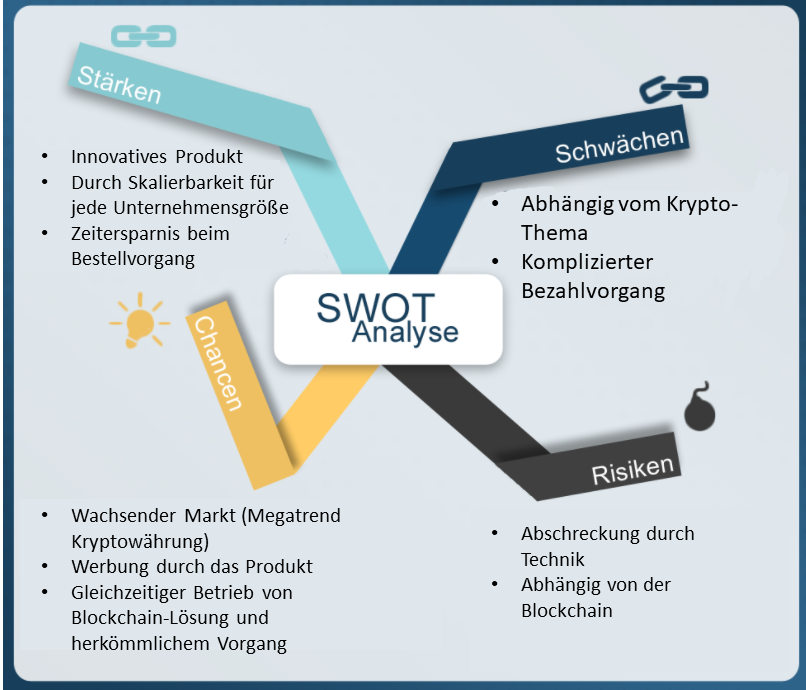
\includegraphics[width=0.9\textwidth]{Bilder/swot_analyse.png}
				\caption[SWOT-Analyse der Protol�sung]{SWOT-Analyse der Protol�sung}
				\label{swot}
			\end{center}
		\end{figure}
	
	
	
	% Ergebnisdiskussion
	%\chapter{Diskussion}

	Neben der Beantwortung der initial formulierten Forschungsfragen wird innerhalb dieses Abschnittes eine komprimierte Analyse von Limitierungen der finalen Themenbetrachtung vorgenommen, welche die Deduktion weiterf�hrender Forschungsans�tze erm�glicht.

	\section{Beantwortung der Forschungsfragen}
	
		Als Leitlinien dieser Arbeit wurden in Abschnitt 1.2 drei zentrale Forschungsfragen formuliert, welche im Folgenden auf Basis der Arbeitsergebnisse diskutiert werden sollen. \\
		
		\noindent\textbf{1. Welche Verfahren zur Analyse von Malware-Implementierungen existieren und welche Relevanz besitzen virtuelle Systeme in diesem Kontext?}\\
		
		\begin{addmargin}[1em]{0em}
			Aus konzeptioneller Perspektive k�nnen die Verfahren zur Examination von Malware-Realisierungen grobgranular in zwei wesentliche Ans�tze differenziert werden. Die \textit{statische Malware-Analyse} realisiert dabei die Evaluation von akquirierten Implementierungs-Fragmenten, um final wesentliche Parameter der Malware-Funktionalit�t rekonstruieren zu k�nnen. Hierzu sind aufgrund der zunehmenden Verbreitung von kryptographischen Algorithmen und Obfuscation-Techniken oftmals extensive Analysen der Quellcode-Exzerpten erforderlich, was final h�ufig in der Notwendigkeit zur manuellen Durchf�hrung resultiert.			
			Der alternative Ansatz der \textit{dynamischen Malware-Analyse} priorisiert hingegen die Analyse des Laufzeit-Verhaltens eines Malware-Implementierung, welches unter Verwendung dedizierter Protokoll- und Monitoringmechanismen detailliert aufgezeichnet wird. Um die Kompromittierung produktiver Systeme weitestgehend ausschlie�en zu k�nnen, werden die dynamischen Analyseans�tze in der Regel innerhalb isolierter Systemumgebungen realisiert.			
			H�ufig wird zur Elimination der individuellen Ansatz-Defizite jedoch ein hybrider Ansatz genutzt, welcher die adaptive Kombination von konzeptionellen Ma�nahmen der statischen und dynamischen Analysemethoden im Hinblick auf die konkrete Analyseproblematik erm�glicht.\\
			\noindent Virtualisierte Systemumgebungen repr�sentieren in diesem Kontext das prim�re Instrument zur Realisierung der konkreten Analysemethoden, indem sie den Betrieb multipler Evaluationsumgebungen sowie deren dynamische Rekonfiguration in strikter Isolation von potentiellen Produktivsysteme offerieren. 
			Aufgrund des koordinierendes Hypervisor-Elements, welches die Separation der emulierten Systemelemente von physischen Hardware-Komponenten realisiert, wird insbesondere die detaillierte Protokollierung von internen Systemaufrufen und etwaiger Netzwerkkommunikation erm�glicht. Unter Verwendung der Hypervisor-Schnittstellen k�nnen dabei wesentlich detaillierte Informationen extrahiert werden, als in physischen Host-System m�glich w�re \textcolor{red}{[11]}. %https://books.google.de/books?id=hrSoCAAAQBAJ&pg=PA17&lpg=PA17&dq=less+vm+detection&source=bl&ots=KqJDeb-Nho&sig=YFe6waQMlr4Qhd1gvDu72OlBQBY&hl=de&sa=X&ved=0ahUKEwjP-rOZ5OzZAhXMjSwKHdzNCUkQ6AEIUTAF#v=onepage&q=gain%20popul&f=false
			Ein weiteres, zentrales Argument zur Nutzung virtueller Systeme im Kontext der Malware-Analyse ist die im Vergleich zu Realsystemen signifikant simplifizierte Konfiguration der Guest-Systeme. Dies erm�glicht die vergleichsweise einfache Konstruktion von komplexen Netzwerk-Umgebungen sowie die Emulation beliebiger Hardware-Subsysteme, sodass der zur Evaluation einer Malware-Implementierung erforderliche Systemkontext individuell konfiguriert werden kann.
			Unter Ber�cksichtigung der zunehmenden Dominanz virtualisierter Systeme in produktiven Einsatzszenarien (exemplarisch sei an dieser Stelle der Webserver-Betrieb referenziert \cite{presentation}) werden auch diese vermehrt Ziel von Malware-Angriffen. Vor dem Hintergrund garantiert die reine Verwendung virtueller Systeme keine Sicherheit vor der m�glichen Kompromittierung des Systems, sodass auch hier \makebox[\linewidth][s]{dedizierte Sicherheitsma�nahmen zur Infektionsabwehr konzipiert werden m�ssen.}
			
		\end{addmargin}	
		\vspace{\baselineskip}
		
		\noindent\textbf{2. Welche systemspezifischen Indizien werden von aktuellen Malware-\\\noindent Implementierungen zur Detektion virtueller Systemumgebungen eingesetzt?}\\
		
		\begin{addmargin}[1em]{0em}
			Auf Basis einer initialen Evaluation der von Virtualisierungs-Implementierungen induzierten System-Anomalien wurden dieser einer grobgranularen Kategorisierung hinsichtlich der intern verwendeten Mechanismen unterzogen. Hierzu wurde eine Differenzierung in vier Subkategorien realisiert, deren Anteile im Verlauf des dedizierten Abschnittes \ref{cha:Virtualisierung} hinsichtlich potentieller Detektionsvektoren analysiert wurden. 
			\noindent Die erste Kategorie priorisiert dabei die Identifikation kompromittierender Namensattribute innerhalb verschiedener Betriebssystem-Implementierungen. In Unix-basierten Systemumgebungen kann diese aufgrund der \textit{everything-is-a-file}-Architektur meist bereits durch die Validierung der Existenz bestimmter Dateifragmente oder Verzeichnisse realisiert werden, wobei zus�tzlich eine extensive Analyse selektiv vorgefilterter Dateiinhalte realisiert werden kann. Das konzeptionelle Analogon zu verteilten, dateibasierten Konfigurationsdaten 
			wird in Windows-Systemen durch die zentralisierte Registry-Datenbank repr�sentiert, welche in ihrer Rolle als universelles Informationselement des Systems auch die Extraktion von potentiellen Virtualisierungs-Indikatoren erlaubt. \\ %wesentlicher Parameter der Systemkonfiguration erlaubt.\\ 
			\noindent Innerhalb der zweiten Kategorie wird die Extraktion von Laufzeit-Attributen aus der virtuellen Hauptspeicher-Komponente forciert. Aufgrund des interaktiven Charakters verschiedener Anteile einer virtuellen Systemumgebung sind innerhalb des System-RAMs oftmals Fragmente der Treiber- oder Hypervisor-Funktionalit�t mit entsprechenden Namensattributen abgelegt, deren Existenz aufgrund der dynamischen Speicherkomposition jedoch nur unter relativ hohem Aufwand validiert werden kann.\\
			Ein zentraler Indikator f�r die Pr�senz von virtualisierten Systemumgebungen wird durch emulierte Hardware-Komponenten repr�sentiert, welche in Kategorie drei analysiert wurden. Zur Realisierung des interaktiven Simulationsbetriebs zwischen dem physischen Host-System und virtualisierten Guest-Instanzen ist die Implementierung spezialisierter Treiberfunktionalit�t erforderlich, wobei die Parameter der hierzu verwendeten Komponenten h�ufig die Deduktion des virtuellen Systemcharakters erlauben.\\ 
			\noindent Final wurde in Kategorie vier die Evaluation von direkten CPU-Instruktionen hinsichtlich ihrer Verwendbarkeit im Kontext der Virtualisierungs-Detektion vorgenommen. Obwohl die Struktur des CPU-Befehlssatzes stark architekturspezifisch ist und somit die feingranulare Anpassung der Detektionsvektoren an das Zielsystem erfordert, bietet sich aufgrund der geringen Interferenzen von CPU-Instruktionen mit Betriebssystem-Implementierungen der Einsatz als additiver Indikator grunds�tzlich an. In der Realit�t werden die hier pr�sentierten Detektionsans�tze zur Ausgleichung individueller Defizite meist kombiniert eingesetzt, wobei insbesondere eine stufenweise Validierung der \makebox[\linewidth][s]{generierten Resultate durch Kategorie-�bergreifende Methoden zu beobachten ist.}
		\end{addmargin}
		\vspace{\baselineskip}
		
		\noindent\textbf{3. Welche Methoden und Verfahren k�nnen zur Optimierung der in einem virtuellen System generierten Analyse-Resultate eingesetzt werden?}\\
		
		\begin{addmargin}[1em]{0em}
			\textcolor{red}{OSTENDORFF}				
		\end{addmargin}
	
	\section{Limitierungen der aktuellen Betrachtung}
	
		Im Rahmen dieser Seminararbeit wurden die Analyseparameter auf die abstrahierte Betrachtung von generischen Malware-Implementierungen ausgerichtet. Die in produktiven Systemumgebungen eingesetzten Derivate weisen jedoch mitunter signifikante Diskrepanzen	 in Implementierung und Verhalten auf; so ist beispielsweise bei hybriden Botnetz-Implementierungen konzeptionsgem�� ein hoher Kommunikationsanteil evident, w�hrend Rootkit-Installationen prim�r verdeckt agieren und dedizierten Detektionma�nahmen daher kaum Angriffsoberfl�che bieten.
		Bei der Konzeption konkreter Analyseumgebungen zur Untersuchung spezifischer Malware-Samples ist daher eine initiale Grobanalyse zur Deduktion der durch das Malware-Derivat verwendeten Evasionstechniken zu empfehlen, welche beispielsweise auf Basis von Untersuchungen verwandter Malware-Familien realisiert werden kann. Darauf aufbauend wird final die feingranulare Adaption der malwareinh�renten Evasionsmethoden zur Konzeption der korrespondierenden Gegenma�nahmen umgesetzt, welche final in der Generierung optimierter Analyse-Resultate resultiert. Diese Form der malwarespezifischen Optimierung der verwendeten Analyseumgebung findet zugunsten einer abstrahierten Perspektive, welche die Abdeckung generischer Malware-Implementierungen erlaubte, im Rahmen dieser Arbeit nur in Ans�tzen Ber�cksichtigung. 
		\noindent In diesem Kontext gestaltet sich insbesondere die Konfiguration automatisierter Analyseumgebungen als �u�erst diffizil, sodass die feingranulare (eventuell malwareindividuelle) Betrachtung einzelner Parameter meist manuell realisiert werden muss. Eine exhaustive Implementierung von Gegen- und Optimierungsma�nahmen ist dabei im Regelfall kaum m�glich, da aufgrund der in Abschnitt \ref{sec:konzept} konstatierten Diversifizierung sowie der zunehmenden Entwicklung von adaptiven Detektionsma�nahmen durch Malware-Entwickler die Komplexit�t kontinuierlich ansteigt. Aus diesem Grund ist auch auf Seiten der Gegenma�nahmen eine auf den Analysekontext angepasste, strategische  Kombination der individuellen Optimierungsmethoden erforderlich, deren Konfiguration individuell auf die untersuchten Malware-Komponenten angepasst werden muss. \\
		\noindent Ausgehend von den im Rahmen der Seminararbeit pr�sentierten, virtualisierten Systemumgebungen wurden durch Sicherheitsanalysten dedizierte Sandbox- und Analysesysteme f�r den Einsatz im Kontext der Malware-Analyse konzipiert. Diese implementieren neben der Hypervisor-basierten Systemisolation auch interne Ma�nahmen zur effektiven Verschleierung der VM-Pr�senz sowie dedizierte Protokoll- und �berwachungsfunktionalit�t. Exemplarisch wurden im Verlauf der initialen Kontextualisierung \textit{Cuckoo} und \textit{Cisco Threat Grid} referenziert, wobei ausgehend von der Schwerpunktsetzung dieser Arbeit auf eine detaillierte Examination der stark spezialisierten Systemumgebungen verzichtet wurde. Aufgrund der zunehmenden Verbreitung von virtuellen Systemen im produktiven Serverbetrieb ist hierbei jedoch eine feingranulare Differenzierung zwischen den System-Kategorien \textit{virtualisierte Systemumgebung} und \textit{dedizierte Analyseumgebung} erforderlich. Aktuelle Malware-Implementierung entwickeln in diesem Kontext gem�� der Ausf�hrungen in Abschnitt \ref{sec:wkt} bereits zuverl�ssige Kompetenzen \cite{fortinet2}. %Quelle:https://blog.fortinet.com/2018/01/03/prevalent-threats-targeting-cuckoo-sandbox-detection-and-our-mitigation
				
		%Aufbauend aus virtualisierten Systemkontext oder Software-Sandbox dedizierte ANalysesysteme konzipiert, welche neben Ma�nahmen zur verschleireung der VM-Pr�senz dedizierte Protokoll- und �berwachungsfunktionalit� implementier. Diese im rhmen dieser arbeit nichtdediizert analysiert; aufgrund zunehmender VErbreitung virtueller Systeme im Kontexdt des produktiven Betriebs feingranulare Differenzuerunig zwischen virtuellen Systemen und dedizieren NAalysesystem erforderlich. Malware entwickelt in diesem kOntext allm�hlich Kompentenzen \textcolor{red}{[11]}%Quelle:https://blog.fortinet.com/2018/01/03/prevalent-threats-targeting-cuckoo-sandbox-detection-and-our-mitigation
		
		\noindent Die zunehmende Omnipr�senz digitaler Systeme manifestiert sich prim�r in den wachsenden Sektoren der Mobilger�te sowie im Kontext des \textit{Internet of Things} (IoT), dessen Forcierung der ubiquit�ren Vernetzung von Alltagsgest�nden die Anzahl zu sch�tzender System massiv erh�ht. Im Rahmen dieser Seminararbeit wurde der Fokus auf die Untersuchung Desktop-basierter Virtualisierungs-L�sungen gelegt, sodass die Malware-Analyse von Mobilger�ten und IoT-Komponenten (sowie potentiellen Beitr�gen der Virtualisierungstechnologie in diesem Bereich) nicht betrachtet wurden. Des Weiteren verf�gen auch moderne Browser-Implementierungen zunehmend �ber isolierte Software-Sandboxes, um die mit potentiell kompromittieren Webinhalten interagierende Browser-Komponente vom Rest des Produktivsystems zu isolieren. Da die Realisierung dieser Mechanismen jedoch weitestgehend systemspezifisch ist, wurden Detektionsma�nahmen f�r diese Technologie im thematischen Kontext der vorliegenden Seminararbeit bewusst nicht ber�cksichtigt.
		
	
	% Konklusion
	\chapter{Konklusion}

Im Folgenden wird zun�chst einmal der Inhalt der Arbeit zusammengefasst \ref{zusa}. Hierbei werden gegebenenfalls auch entsprechende Ergebnisse aufgezeigt. Anschlie�end werden potentielle Ausblicke in zuk�nftige Verwendung gegeben beziehungsweise Vermutungen ge�u�ert, was die Technologie erm�glichen k�nnte \ref{ausb}.

\section{\label{zusa}Zusammenfassung}

In Kapitel \ref{chap:1einleitung} wurde zun�chst an das Thema herangef�hrt. Hierzu z�hlte die schemenhafte Einordnung des Wertes von Daten sowie das anschlie�ende Begr�nden anhand eines Beispiels, warum solche Daten wichtig sind und es die M�glichkeit geben sollte diese auf Korrektheit zu pr�fen. Au�erdem wurde die Grundfunktionalit�t einer Blockchain kurz angerissen und die wohl bekanntesten Vertreter genannt. In Kapitel \ref{chap:2grundlagen} wurden die Grundlagen erl�utert. Hierzu geh�rten der Begriff des Krypto Hashes, der Unterschied zwischen zentralisierten und verteilten beziehungsweise Peer-to-Peer Netzen, das beleuchten von public-/privat-Key Verfahren beziehungsweise asymmetrische Kryptographie sowie die Einordnung der wohl bekanntesten Kryptow�hrungen. Dabei handelte es sich um Bitcoin und Ethereum, welche als Abschluss des Kapitels verglichen wurden. In Kapitel \ref{chap:3methodik} wurde die methodische Herangehensweise der Arbeit vorgestellt. Dies beinhaltete sowohl gruppeninterne organisatorische Aspekte, als auch zur Durchf�hrung der Arbeit notwendige beziehungsweise geplante Schritte. Zus�tzlich wurden die Grundlagen beziehungsweise Hintergr�nde der einzelnen Aspekte kurz beleuchtet. Gruppenintern betraf dies beispielsweise das Kanban-Tool Trello, welches die Gruppe verwendete, um die Arbeiten zu planen und Einsicht in den Stand anderer Teilarbeiten zu haben sowie permanent einsch�tzen zu k�nnen in welchem Arbeitsstadium sich die Gruppe grade befand. Eher auf das Projekt selbst bezogen waren eine Machbarkeitsstudie ob die Idee tats�chlich so umsetzbar sei und eine Risikoanalyse. Die tats�chliche Umsetzung dieser Ma�nahmen folgten im n�chsten Kapitel. Bei diesem Kapitel handelt es sich um Kapitel \ref{chap:4szenario}. Hier wurde zuerst ein betriebswirtschaftlicher Kontext hergestellt beziehungsweise erl�utert. Darauf folgte die Darstellung des Fallbeispiels Whoppercoin Burger King. Der Hauptteil des Kapitels besteht der Beschreibung von Use Cases im Gastronomie-Kontext. Dort wurden neben der Erl�uterung der Kunden- und Betreiberperspektive auch die erw�hnte Machbarkeitsstudie und Risikoanalyse durchgef�hrt. Das Kapitel endet schlie�lich mit einem Interview mit der UniBar. Im folgenden und letzten Inhaltskapitel \ref{chap:5proto} wurde die Entwicklung eines Prototypen auf Webbasis beschrieben. Hierf�r wurden au�erdem die Grundlagen beziehungsweise die Bedeutung von Smart Contracts erl�utert. Im Verlauf des Kapitels wird kurzer Einblick in den Quellcode gegeben sowie grob die Funktionalit�t der Applikation beschrieben. Das Kapitel schlie�t mit bildlichen Darstellungen der App beziehungsweise des Frontends.

\section{\label{ausb}Ausblick} 

In dieser Arbeit ist es gelungen einen vorl�ufigen Prototypen zu entwerfen, der geforderte Funktionalit�ten simulierend abbilden kann. Auch die Machbarkeitsstudie viel positiv aus. Somit wurde sowohl theoretisch als auch ansatzweise praktisch gezeigt, dass eine tats�chliche Umsetzung m�glich sein sollte. Es ist durchaus denkbar, dass bei der eventuellen Weiterf�hrung in zuk�nftigen Projekten eine verwertbare beziehungsweise einsetzbare Software produziert werden k�nnte. Grade f�r kleinere Unternehmen biete es sich an solche dezentralen L�sungen zu w�hlen, da sie das Unternehmen selbst entlasten w�rden, was aber nicht hei�t, dass die Technologie f�r gro�e Unternehmen keinen Mehrwert bringen k�nnte. Bei der vorgestellten Technologie handelt es sich um brandaktuelle Technologie beziehungsweise in einigen Forschungseinrichtung behandelte Konzepte. Dies bedeutet allerdings, dass man sich, um das Thema zumindest ansatzweise erfassen zu k�nnen ausgiebig damit auseinandersetzen muss. Hierf�r haben viele Menschen aber einfach nicht die Zeit und befinden sich zus�tzlich in einem komplett anderen T�tigkeitsfeld. Im Rahmen der Arbeit wurde Interviews durchgef�hrt. Bei diesen wurde die eben ge�u�erte Vermutung best�tigt, dass den Betroffenen das n�tige Fachwissen fehlt um den potentiellen technischen Mehrwert erfassen zu k�nnen. Wenn die Technologie sich etablieren soll ist es sinnvoll dar�ber nachzudenken vorher erst einmal eine Art technische Aufkl�rung zu betreiben, damit die Betroffenen wissen, womit sie es wirklich zu tun haben und was es ihnen bringen k�nnte diese Technologie zu verwenden. In dieser Arbeit wurde exemplarisch die Gastronomie ausgew�hlt, womit es sich um einen allt�glichen Lebensbereich vieler handelt. Die aufgezeigten Funktionalit�ten lassen sich allerdings auf viele andere Bereiche, in welchen Transaktionen durchgef�hrt werden, �bertragen und die Technologie ist nat�rlich nicht auf diese Spate beschr�nkt. Um ein Beispiel zu nennen, welches jetzt nicht, wie das in dieser Arbeit gelieferte Beispiel, direkter Teil der Gastronomie w�re, k�nnte beispielsweise ein Logistikunternehmen, was hier den Zulieferer abbilden k�nnte herangezogen werden. Wenn die Gesch�fte zwischen Zulieferer und Restaurant oder �hnlichem nun mit einer �hnlichen Technologie, wie im Demonstrator gezeigt wurde, Vertr�ge abschlie�en w�rde w�re es beispielsweise nicht mehr notwendig, dass tats�chlich unterschriebene Vertr�ge existieren. Dies w�rde gegebenenfalls den Postweg, oder die tats�chliche Anwesenheit der beiden Vertragsparteien nicht weiter ben�tigen, da diese Vertr�ge auch aus der Entfernung abgeschlossen werden k�nnten. Die Anwendungsf�lle sind lediglich durch die Kreativit�t eingeschr�nkt. Ob es dazu kommt kann man weder best�tigen, noch widerlegen. Ein potentieller Nutzen der Technologie wurde aufgezeigt. Es ist zumindest denkbar, dass das ein oder andere Unternehmen sich dessen in zuk�nftigen Projekten bedienen wird.
	
	\begin{appendices}
		\renewcommand\chaptername{Appendix}
		%\clearpage
%\vspace*{\fill}
%\thispagestyle{empty}
%\begin{minipage}{1\textwidth}%
%	\chapter{Tabelle NSE SKRIPTE REIHENFOLGE ABER NOCH TAISCHEN LEL}
%\end{minipage}
%\vfill % equivalent to \vspace{\fill}
%\clearpage
%\newpage
%
%\clearpage
%\thispagestyle{plain}
%
%
%\noindent\Large\textbf{Tabelle NSE SKRIPTE}
%
%\renewcommand\arraystretch{1.0}% (MyValue=1.0 is for standard spacing)
%
%\begin{table}[h]
%	
\clearpage
\vspace*{\fill}
	\begin{minipage}{1\textwidth}
		\chapter[Transkript der Interviews]{Transkript der Interviews}\label{anhang}
	\end{minipage}
\vfill % equivalent to \vspace{\fill}
\clearpage


\newpage
%\clearpage
%\thispagestyle{empty}
		
\textbf{{\large Ablauf Interview:}}

\begin{enumerate}
	\item Fragen zur Blockchain (Wissensstand: Was sind Kryptow�hrungen? Was ist die Blockchain? Anwendungsgebiete?)
	\item Erkl�rung der Blockchain, Erkl�rung von Ethereum 
	\item Fragen �ber die derzeitige Situation der Bar (Bestellvorgang, Bezahlung, Webauftritt)
	\item Vorstellung des Szenarios 
	\item Fragen �ber das Szenario: Vorstellbar, Heute Umsetzbar (Begr�ndung f�r ja und nein)
	\item Abschlie�ende Worte
\end{enumerate}

\newpage

\textbf{{\large Landgasthof alter Bahnhof (Rohrberg)}}

\begin{enumerate}
	\item Fragen zur Blockchain (Wissensstand: Was sind Kryptow�hrungen? Was ist die Blockchain? Anwendungsgebiete?)
	\begin{itemize}
		\item Name schon mal geh�rt
		\item Kein Wissen �ber genaue Bedeutung und Anwendung
	\end{itemize}
	\item Erkl�rung der Blockchain, Erkl�rung von Ethereum 
	\begin{itemize}
		\item Kurze Erkl�rung �ber die Technologie und Anwendungsm�glichkeiten
	\end{itemize}
	\item Fragen �ber die derzeitige Situation der Bar (Bestellvorgang, Bezahlung, Webauftritt)
	\begin{itemize}
		\item Herk�mmlicher Bestellvorgang
		\item Speisekarte als Buch, indem Speisen und Getr�nke mitsamt Preisen stehen
		\item Bar und Kartenzahlung m�glich
		\item Webauftritt �ber diverse Drittanbieter, keine eigene Homepage
	\end{itemize}
	\item Vorstellung des Szenarios
	\begin{itemize}
		\item Kurze Erkl�rung des Szenarios
		\item Erl�uterung der Vor- und Nachteile
	\end{itemize} 
	\item Fragen �ber das Szenario: Vorstellbar, Heute Umsetzbar (Begr�ndung f�r ja und nein)
	\begin{itemize}
		\item Interessantes Thema
		\item K�nnte eines Tages die Zahlungsmethode �ndern
		\item Heute nicht vorstellbar (zu wenig wissen dar�ber, kaum jemand nutzt es)
		\item F�r Werbezwecke aufgrund der genannten Gr�nde nicht nutzbar
		\item Kosten-Nutzen nicht positiv			
	\end{itemize}
	\item Abschlie�ende Worte
	\begin{itemize}
		\item l�ndliche Gegend folgt selten neuen Trends
		\item setzt auf altbew�hrtes
	\end{itemize}
\end{enumerate}

\newpage

\textbf{{\large Taverne Artemis  (Ottobrunn)}}

\begin{enumerate}
	\item Fragen zur Blockchain (Wissensstand: Was sind Kryptow�hrungen? Was ist die Blockchain? Anwendungsgebiete?)
	\begin{itemize}
		\item Im groben informiert
		\item Durch Nachrichten in den Fokus geraten
		\item F�r zu kompliziert erachtet
	\end{itemize}
	\item Erkl�rung der Blockchain, Erkl�rung von Ethereum 
	\begin{itemize}
		\item Kurze Erkl�rung �ber die Technologie und Anwendungsm�glichkeiten
	\end{itemize}
	\item Fragen �ber die derzeitige Situation der Bar (Bestellvorgang, Bezahlung, Webauftritt)
	\begin{itemize}
		\item Herk�mmlicher Bestellvorgang (Kellner geht zum Tisch und nimmt pers�nlich Bestellung auf)
		\item Speisekarte als Buch, Extrablatt f�r Sonderangebote/Tageskarte
		\item Bar und Kartenzahlung m�glich, junge Menschen h�ufiger mit EC-Karte
		\item Eigener Webauftritt mit kleiner Homepage
	\end{itemize}
	\item Vorstellung des Szenarios
	\begin{itemize}
		\item Kurze Erkl�rung des Szenarios
		\item Erl�uterung der Vor- und Nachteile
	\end{itemize} 
	\item Fragen �ber das Szenario: Vorstellbar, Heute Umsetzbar (Begr�ndung f�r ja und nein)
	\begin{itemize}
		\item Interessantes Thema, aber sehr komplex und nur f�r technikaffine
		\item Heute nicht vorstellbar (zu wenig wissen dar�ber, kaum jemand nutzt es in der Gegend)
		\item F�r Werbezwecke vielleicht nutzbar, wenn keine Kosten entstehen
		
	\end{itemize}
	\item Abschlie�ende Worte
	\begin{itemize}
		\item Gerne mit fertigem Produkt wiederkommen
		\item Wenn Kryptothema interessant bleibt, wird es viel ver�ndern
	\end{itemize}
\end{enumerate}

\newpage

\textbf{{\large Die 2  (Neubiberg)}}

\begin{enumerate}
	\item Fragen zur Blockchain (Wissensstand: Was sind Kryptow�hrungen? Was ist die Blockchain? Anwendungsgebiete?)
	\begin{itemize}
		\item Kryptow�hrungen meist eine eigene Blockchain, funktioniert dann ein virtueller "Ledger", also eine Art Bestandsbuch, in dem jede Transaktion gespeichert wird
		\item hervorragend als dezentrale W�hrung
		\item direkte Verbindung zwischen allen Teilnehmern des Netzwerkes aufgebaut und somit ist es einer einzelnen Institution nicht m�glich, den Geldfluss zu korrumpieren
		\item Anwendungsgebiete besonders beim "Digital Cash" und Micro-Transaktionen
		\item Durch Blockchain kann Geld relativ schnell, z�gig und sicher  Benutzer wechseln
	\end{itemize}
	\item Erkl�rung der Blockchain, Erkl�rung von Ethereum 
	\begin{itemize}
		\item entf�llt, da umfangreiches Wissen vorhanden
	\end{itemize}
	\item Fragen �ber die derzeitige Situation der Bar (Bestellvorgang, Bezahlung, Webauftritt)
	\begin{itemize}
		\item normaler Bestellvorgang 
		\item m�glich mit EC-Karte und Bargeld zu bezahlen
		\item mehr Kunden nutzten die Kartenzahlung, da Bargeld �fter vergessen
		\item umst�ndlicher als mit Bargeld, da der Bezahlvorgang mit dem EC-Kartenger�t wesentlich l�nger dauert
		\item eigener Webauftritt
	\end{itemize}
	\item Vorstellung des Szenarios
	\begin{itemize}
		\item Kurze Erkl�rung des Szenarios
		\item Erl�uterung der Vor- und Nachteile
	\end{itemize} 
	\item Fragen �ber das Szenario: Vorstellbar, Heute Umsetzbar (Begr�ndung f�r ja und nein)
	\begin{itemize}
		\item viele Menschen vertrauen dem Blockchain-Prinzip nicht (Kursschwankungen)
		\item Marketing Technisch k�nnte es nat�rlich vorteilhaft sein, wenn man zu den "ersten" geh�rt
		\item Art Alleinstellungsmerkmal - "Cool"
		\item Wenn Kosten f�r Anschaffung nicht zu hoch sind, h�rt sich das auf jeden Fall interessant an
		
	\end{itemize}
	\item Abschlie�ende Worte
	\begin{itemize}
		\item definitiv nicht, dass die Blockchaintechnologie in naher Zukunft das Bargeld abl�st. 
		\item Bargeld auch verwenden wenn der Akku mal leer ist oder man kein Netz hat
	\end{itemize}
\end{enumerate}

\newpage

\textbf{{\large Unicasino  (Neubiberg)}}

\begin{enumerate}
	\item Fragen zur Blockchain (Wissensstand: Was sind Kryptow�hrungen? Was ist die Blockchain? Anwendungsgebiete?)
	\begin{itemize}
		\item durch Whitepaper Bitcoin/Blockchain und Ethereum und News einigerma�en 'tiefgehendes' Verst�ndnis der Technologie/technischen Komponenten 
		\item Blockchain: Koh�rente, Konsistenz- und Integrit�tsichernde Transaktionstechnologie
		\item Kryptow�hrungen: Basierend auf Blockchain dezentrale, partiell anonymisierbare Transaktionen  m�glich; 
		\item Verzicht auf zentrale Vertrauensinstanz (wie beispielsweise einer Bank) 
		\item soll Regulierung und Kontrolle erschweren
		
	\end{itemize}
	\item Erkl�rung der Blockchain, Erkl�rung von Ethereum 
	\begin{itemize}
		\item Kurze Erkl�rung �ber die Technologie und Anwendungsm�glichkeiten
	\end{itemize}
	\item Fragen �ber die derzeitige Situation der Bar (Bestellvorgang, Bezahlung, Webauftritt)
	\begin{itemize}
		\item Bezahlung �ber Bargeld oder EC-Karte
		\item Unterschiedliche Bestellungs-/Bezahlvorg�nge (Restaurant und Bar)
		\begin{itemize}
			\item Bar erst bezahlen, dann Getr�nk
			\item Restaurant erst Essen/Trinken, am Ende bezahlen (Trinkgeldaspekt)
		\end{itemize}
		\item Bestellvorgang manuell, Bargeld eventuell hinderlich/unhandlich
		\item Website f�r allgemeine Informationen, Werbung f�r Veranstaltungen und Onlinereservierungen
		
	\end{itemize}
	\item Vorstellung des Szenarios
	\begin{itemize}
		\item Kurze Erkl�rung des Szenarios
		\item Erl�uterung der Vor- und Nachteile
	\end{itemize} 
	\item Fragen �ber das Szenario: Vorstellbar, Heute Umsetzbar (Begr�ndung f�r ja und nein)
	\begin{itemize}
		\item Da Mobilger�t immer dabei, Bezahloption naheliegend
		\item Mit Wallet auf Handy Transaktionen einfach zu realisieren
		\item Gerade im aktuellen Blockchain-Hype Potential nutzbar ('Hipster'-Bar)
		\item Webauftritt heute eigentlich obligatorisch, Integration Bezahlfunktionalit�t sinnvoll
		\item Feinheiten der Umsetzung schwierig (Wie findet erste Authentifizierung des Nutzers statt?)
		\item Umsetzbarkeit wohl nur aus marketing-technischer Sicht sinnvoll, Konzept bringt weder Betreiber noch Endkunde signifikante Komfort-Vorteil
		\item Umsetzung nur als Trend-Konzept, Technologie liefert keinen produktiver Beitrag 
		
		
	\end{itemize}
	\item Abschlie�ende Worte
	\begin{itemize}
		\item Blockchain-Technologie in der praktischen Verwendbarkeit stark limitiert
		\item Insbesondere Skalierbarkeit und Stabilit�t der W�hrungs-Anteile kritisch
	\end{itemize}
\end{enumerate}

\newpage

\textbf{{\large La Ciacolada  (Neubiberg)}}

\begin{enumerate}
	\item Fragen zur Blockchain (Wissensstand: Was sind Kryptow�hrungen? Was ist die Blockchain? Anwendungsgebiete?)
	\begin{itemize}
		\item Kryptow�hrungen sind Online W�hrungen, die unf�lschbar sind 
		\item Nur Bitcoin aus den Medien
		\item Blockchain ist die Technologie, die hinter Bitcoin steht
		\item 
	\end{itemize}
	\item Erkl�rung der Blockchain, Erkl�rung von Ethereum 
	\begin{itemize}
		\item Kurze Erkl�rung �ber die Technologie und Anwendungsm�glichkeiten (aufbauend auf dem vorhandenen Wissen)
	\end{itemize}
	\item Fragen �ber die derzeitige Situation der Bar (Bestellvorgang, Bezahlung, Webauftritt)
	\begin{itemize}
		\item Website f�r allgemeine Informationen, Werbung f�r Veranstaltungen und Onlinereservierungen
		\item Kellner nimmt die Bestellung auf und notiert diese auf einem Zettel (also alles analog)
		\item kennt im Regelfall die Preise und rechnet den Gesamtpreis dann ab
		\item Vertrauensbasis gegen�ber den Kellnern gearbeitet, da diese leicht betr�gen k�nnten
		\item Bezahlt wird regul�r entweder mit Bargeld oder Bankkarte
	\end{itemize}
	\item Vorstellung des Szenarios
	\begin{itemize}
		\item Kurze Erkl�rung des Szenarios
		\item Erl�uterung der Vor- und Nachteile
	\end{itemize} 
	\item Fragen �ber das Szenario: Vorstellbar, Heute Umsetzbar (Begr�ndung f�r ja und nein)
	\begin{itemize}
		\item Heute nicht vorstellbar (zu wenig wissen dar�ber)
		\item jetziges System funktioniert
		\item theoretisch aber umsetzbar, da jeder Smartphone besitzt
		
	\end{itemize}
	\item Abschlie�ende Worte
	\begin{itemize}
		\item keine
	\end{itemize}
\end{enumerate}

\newpage

\textbf{{\large Santorino (Naumburg)}}

\begin{enumerate}
	\item Fragen zur Blockchain (Wissensstand: Was sind Kryptow�hrungen? Was ist die Blockchain? Anwendungsgebiete?)
	\begin{itemize}
		\item bereits schon etwas �ber Kryptow�hrungen geh�rt
		\item Kryptow�hrungen in den letzten Jahren gro�er Hype 
		\item aber auch Beginn der Regulierung bzw. Verbot oder strikterer Umgang durch Banken/Regierungen
		\item Begriff Blockchain nur in Zusammenhang mit Kryptow�hrungen geh�rt
		
	\end{itemize}
	\item Erkl�rung der Blockchain, Erkl�rung von Ethereum 
	\begin{itemize}
		\item Kurze Erkl�rung �ber die Technologie und Anwendungsm�glichkeiten (aufbauend auf vorhandenem Wissen)
	\end{itemize}
	\item Fragen �ber die derzeitige Situation der Bar (Bestellvorgang, Bezahlung, Webauftritt)
	\begin{itemize}
		\item Bedienung kommt zum Kunden, nimmt Bestellung auf
		\item Getr�nke/Speisen auf Zettel beim Kunden festgehalten
		\item Bezahlung vor Verlassen des Lokals in bar oder mit EC-Karte
		\item kein eigener Webauftritt vorhanden, auch nicht notwendig (Stammkunden)
		
	\end{itemize}
	\item Vorstellung des Szenarios
	\begin{itemize}
		\item Kurze Erkl�rung des Szenarios
		\item Erl�uterung der Vor- und Nachteile
	\end{itemize} 
	\item Fragen �ber das Szenario: Vorstellbar, Heute Umsetzbar (Begr�ndung f�r ja und nein)
	\begin{itemize}
		\item nicht vorstellbar, dass es zum Einsatz kommt
		\item Lokal ist auf dem Dorf, viele �ltere G�ste
		\item die wenigsten kennen sich damit aus
		\item Technik m�sste angeschafft werden
		\item kein Mehrwert dadurch
		
		
	\end{itemize}
	\item Abschlie�ende Worte
	\begin{itemize}
		\item keine
	\end{itemize}
\end{enumerate}


	\end{appendices}
	
	
	% Literaturverzeichnis	
	\nocite{*}
	\bibliographystyle{unsrt}
	\bibliography{Literatur}
	        % Bibtex-Datei "Literatur.bib" einbinden
	%\bibliographystyle{plaindin}
	
	
%	
\thispagestyle{empty}
\clearpage
\hbox{}\newpage
%	\thispagestyle{empty}

\end{document}

% Quellen:
% [0]: https://www.bsi.bund.de/SharedDocs/Downloads/DE/BSI/Publikationen/Lageberichte/Lagebericht2016.pdf;jsessionid=E4F12AF765F2552CC408B38D56EE4E4C.1_cid360?__blob=publicationFile&v=5
% [1]: http://www.tagesspiegel.de/wirtschaft/cyberkriminalitaet-verfassungsschutz-und-wirtschaft-schlagen-alarm-50-milliarden-schaden/19730102.html
% [2]: https://www.esg.de/unternehmen/